% lecture9.tex -- GENERATED by build_L9.py from L9_numbers.json; do not edit by hand.
\documentclass[10pt,aspectratio=169,t]{beamer}
% =============================================================================
% nn_preamble.tex -- shared Beamer preamble of Neural Networks and Deep Learning (NN)
% Used by every lecture: lectures/Lk/lecturek.tex does
%   \documentclass[10pt,aspectratio=169,t]{beamer}
%   % =============================================================================
% nn_preamble.tex -- shared Beamer preamble of Neural Networks and Deep Learning (NN)
% Used by every lecture: lectures/Lk/lecturek.tex does
%   \documentclass[10pt,aspectratio=169,t]{beamer}
%   % =============================================================================
% nn_preamble.tex -- shared Beamer preamble of Neural Networks and Deep Learning (NN)
% Used by every lecture: lectures/Lk/lecturek.tex does
%   \documentclass[10pt,aspectratio=169,t]{beamer}
%   \input{../common/nn_preamble}
%   \nnlecture{k}{Lecture title}
% Logos live in lectures/common/logos/, charts in lectures/Lk/charts/.
% Do NOT add \hfuzz / \vfuzz / \hbadness here: overfull boxes must be fixed, not hidden.
% =============================================================================

\usetheme{default}
\setbeamersize{text margin left=7mm, text margin right=7mm}

% ---------------------------------------------------------------- packages
\usepackage[utf8]{inputenc}
\usepackage[T1]{fontenc}
\usepackage{lmodern}
\usepackage{amsmath, amssymb}
\usepackage{mathtools}
\usepackage{bm}
\usepackage{tikz}
\usetikzlibrary{arrows.meta, positioning, calc, shapes.misc}
\usepackage{booktabs}
\usepackage{array}
\usepackage{graphicx}
\usepackage{colortbl}
\usepackage{xcolor}
\usepackage{multicol}
\hypersetup{colorlinks=true, linkcolor=MainBlue, urlcolor=MainBlue, citecolor=MainBlue}
\graphicspath{{../common/logos/}}   % charts are included with their language folder: charts/en/, charts/ro/

% ---------------------------------------------------------------- colours
\definecolor{MainBlue}{RGB}{26, 58, 110}
\definecolor{IDAred}{RGB}{205, 0, 0}
\definecolor{DarkGray}{RGB}{51, 51, 51}
\definecolor{FooterGray}{RGB}{100, 100, 100}
\definecolor{BlockGray}{RGB}{236, 238, 242}
\definecolor{KeynoteGray}{RGB}{218, 218, 218}
\definecolor{Crimson}{RGB}{190, 40, 50}
\definecolor{Forest}{RGB}{30, 110, 50}
\definecolor{Bitter}{RGB}{214, 150, 20}
% chart palette (same hex values and order as lectures/common/nn_plot.py SERIES)
\definecolor{Ser1}{HTML}{2A78D6}
\definecolor{Ser2}{HTML}{EB6834}
\definecolor{Ser3}{HTML}{1BAF7A}
\definecolor{Ser4}{HTML}{EDA100}
\definecolor{Ser5}{HTML}{E87BA4}
\definecolor{Ser6}{HTML}{008300}
\definecolor{Ser7}{HTML}{6250D6}
\definecolor{Ser8}{HTML}{E34948}

\setbeamertemplate{background}{%
  \begin{tikzpicture}[remember picture, overlay]
    \shade[shading=axis, shading angle=315, top color=white, bottom color=KeynoteGray]
      (current page.south west) rectangle (current page.north east);
  \end{tikzpicture}}
\setbeamercolor{background canvas}{bg=}
\setbeamercolor{structure}{fg=MainBlue}
\setbeamercolor{normal text}{fg=DarkGray}
\setbeamercolor{title}{fg=IDAred}
\setbeamercolor{frametitle}{fg=IDAred, bg=}
\setbeamercolor{block title}{bg=MainBlue, fg=white}
\setbeamercolor{block body}{bg=BlockGray, fg=DarkGray}
\setbeamercolor{block title alerted}{bg=Crimson, fg=white}
\setbeamercolor{block body alerted}{bg=Crimson!7, fg=DarkGray}
\setbeamercolor{block title example}{bg=Forest, fg=white}
\setbeamercolor{block body example}{bg=Forest!7, fg=DarkGray}
\setbeamercolor{item}{fg=MainBlue}
\setbeamerfont{frametitle}{size=\large, series=\bfseries}
\setbeamerfont{block title}{size=\small, series=\bfseries}
\setbeamertemplate{blocks}[rounded][shadow=false]
\setbeamertemplate{itemize item}{\color{MainBlue}$\boxdot$}
\setbeamertemplate{itemize subitem}{\color{MainBlue}\scriptsize$\blacktriangleright$}
% compact two-level lists: level 1 = main point, level 2 = details (no text outside bullets)
\setbeamerfont{itemize/enumerate subbody}{size=\footnotesize}
\setlength{\leftmargini}{1.1em}
\setlength{\leftmarginii}{1.1em}
\setbeamertemplate{itemize/enumerate body begin}{\setlength{\topsep}{0pt}\setlength{\partopsep}{0pt}\setlength{\parskip}{0pt}}
\setbeamertemplate{itemize/enumerate subbody begin}{\setlength{\topsep}{0pt}\setlength{\partopsep}{0pt}\setlength{\itemsep}{0pt}\vspace{-0.4ex}}

\setbeamertemplate{enumerate item}{\color{MainBlue}\insertenumlabel.}
\setlength{\leftmargini}{1.3em}
\setlength{\leftmarginii}{1.2em}
\setbeamertemplate{navigation symbols}{}
\setbeamertemplate{section in toc}{\color{MainBlue}$\blacktriangleright$~\inserttocsection}
\setbeamertemplate{caption}{\raggedright\insertcaption\par}
% frame subtitle = precise citation line under the claim title (Weron style)
\setbeamerfont{framesubtitle}{size=\footnotesize}
\setbeamercolor{framesubtitle}{fg=FooterGray}
% outline that reappears at every section with the current section highlighted
\setbeamertemplate{section in toc shaded}[default][35]
\setbeamertemplate{subsection in toc shaded}[default][35]
\setbeamertemplate{subsection in toc}{\leavevmode\leftskip=2.2em\color{DarkGray}\small\inserttocsubsection\par}
\AtBeginSection[]{{\begin{frame}{\txtoutline}\vspace{2mm}\small
  \tableofcontents[currentsection,hideothersubsections]\end{frame}}}

% ---------------------------------------------------------------- head and foot
\setbeamertemplate{headline}{%
  \vskip10pt%
  \hbox to \paperwidth{\hskip0.5cm%
    {\small\color{FooterGray}\renewcommand{\hyperlink}[2]{##2}\insertsectionhead}%
    \hfill\textcolor{FooterGray}{\small\insertframenumber}\hskip0.5cm}%
  \vskip4pt{\color{FooterGray}\hrule height 0.4pt}}
% footer as in the other courses (MFM, SFM): course name on the left, small sparkline on the right
\setbeamertemplate{footline}{%
  {\color{FooterGray}\hrule height 0.4pt}\vskip4pt%
  \hbox to \paperwidth{\hskip0.5cm%
    \textcolor{FooterGray}{\small\txtcourse}%
    \hfill\raisebox{-0.1em}{\begin{tikzpicture}[x=0.08em, y=0.08em, line width=0.4pt]
      \draw[FooterGray] (0,3) -- (1,4) -- (2,3.5) -- (3,5) -- (4,4) -- (5,6) -- (6,5.5) -- (7,4) -- (8,5) -- (9,7) -- (10,6) -- (11,5) -- (12,6.5) -- (13,8) -- (14,7) -- (15,6) -- (16,7.5) -- (17,9) -- (18,8) -- (19,7) -- (20,8.5) -- (21,10) -- (22,9) -- (23,8) -- (24,9.5);
    \end{tikzpicture}}\hskip0.5cm}%
  \vskip6pt}

% ---------------------------------------------------------------- title page
\defbeamertemplate*{title page}{nn}[1][]{%
  \vspace{0.15cm}
  \begin{center}
    \href{https://www.ase.ro}{
\includegraphics[height=0.9cm]{ase_logo.png}}\hspace{0.3cm}%
    \href{https://ipe.ro/new}{
\includegraphics[height=0.9cm]{acad_logo.png}}\hspace{0.3cm}%
    \href{https://theida.net}{
\includegraphics[height=0.9cm]{ida_logo.png}}\hspace{0.3cm}%
    \href{https://blockchain-research-center.com}{
\includegraphics[height=0.9cm]{brc_logo.png}}\hspace{0.3cm}%
    \href{https://www.ai4efin.ase.ro}{
\includegraphics[height=0.9cm]{ai4efin_logo.png}}\hspace{0.3cm}%
    \href{https://www.digital-finance-msca.com}{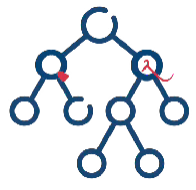
\includegraphics[height=0.9cm]{msca_logo.png}}%
  \end{center}
  \vspace{0.45cm}
  \begin{center}
    \begin{minipage}{0.1\textwidth}\centering
      \href{https://quantlet.com}{
\includegraphics[height=0.9cm]{ql_logo.png}}\end{minipage}%
    \begin{minipage}{0.78\textwidth}\centering
      {\Large\bfseries\usebeamercolor[fg]{title}\inserttitle}\par\vspace{0.25cm}
      {\large\usebeamercolor[fg]{title}\insertsubtitle}\end{minipage}%
    \begin{minipage}{0.1\textwidth}\centering
      \href{https://quantinar.com}{
\includegraphics[height=0.9cm]{qr_logo.png}}\end{minipage}
  \end{center}
  \vfill
  \hspace{0.4cm}{\bfseries\insertauthor}\par\vspace{0.12cm}
  \hspace{0.4cm}\begin{minipage}[t]{0.92\textwidth}\raggedright\footnotesize\insertinstitute\end{minipage}
  \par\vspace{0.4cm}}

% ---------------------------------------------------------------- lecture metadata
\newcommand{\nnshort}{}
\newcommand{\nnnb}{notebooks}
\newcommand{\nnrepo}{https://github.com/danpele/NEURAL_BIZ/tree/main}
% language-dependent labels (English default; \nnromanian switches to Romanian, call it before \nnlecture)
\newcommand{\txtcourse}{Neural Networks and Deep Learning}
\newcommand{\txtlecture}{Lecture}
\newcommand{\txtoutline}{Outline}
\newcommand{\txtintuition}{In one sentence:}
\newcommand{\txtjob}{In practice:}
\newcommand{\txttry}{Experiment yourself:}
\newcommand{\txtwhere}{where}
\newcommand{\txtsim}{SIMULATED DATA (teaching illustration)}
\newcommand{\txtnbsuffix}{}
\newcommand{\txtinstitute}{Bucharest University of Economic Studies (ASE), Department of Statistics and Econometrics\\
    Romanian Academy, Institute for Economic Forecasting (IPE)\\
    IDA Institute Digital Assets \textbullet\ AI4EFin \textbullet\ MSCA Digital Finance}
\newcommand{\nnromanian}{%
  \renewcommand{\txtcourse}{Rețele neuronale și deep learning}%
  \renewcommand{\txtlecture}{Cursul}%
  \renewcommand{\txtoutline}{Cuprins}%
  \renewcommand{\txtintuition}{Pe scurt:}%
  \renewcommand{\txtjob}{În practică:}%
  \renewcommand{\txttry}{Exercițiu practic:}%
  \renewcommand{\txtwhere}{unde}%
  \renewcommand{\txtsim}{DATE SIMULATE (doar pentru ilustrare)}%
  \renewcommand{\txtnbsuffix}{\string_ro}%
  \renewcommand{\txtinstitute}{Academia de Studii Economice din București (ASE), Departamentul de Statistică și Econometrie\\
    Academia Română, Institutul de Prognoză Economică (IPE)\\
    IDA Institute Digital Assets \textbullet\ AI4EFin \textbullet\ MSCA Digital Finance}}
\newcommand{\nnlecture}[2]{%
  \renewcommand{\nnshort}{\txtlecture\ #1}%
  \renewcommand{\nnnb}{notebooks/L#1\string_notebook\txtnbsuffix.ipynb}%
  \title[NN]{\txtcourse}%
  \subtitle{\txtlecture\ #1: #2}%
  \author{Prof.\ dr.\ Daniel Traian PELE}%
  \institute{\txtinstitute}%
  \date{}}

% ---------------------------------------------------------------- teaching blocks (one message per frame)
% \intuition{one plain sentence}  ->  formula with every symbol defined  ->  real-data example  ->  \manager{one line}
\newcommand{\intuition}[1]{\begin{itemize}\item {\color{MainBlue}\textbf{\txtintuition}}~#1\end{itemize}\vspace{0.6mm}}
\newcommand{\manager}[1]{\colorbox{Forest!10}{\parbox{\dimexpr\linewidth-2\fboxsep\relax}{\footnotesize
  \begin{itemize}\setlength{\itemsep}{0pt}\item \textbf{\color{Forest}\txtjob}~#1\end{itemize}}}}
% Experiment yourself: pointer to the matching notebook section
\newcommand{\tryit}[1]{{\scriptsize\href{\nnrepo/\nnnb}{%
  \raisebox{-0.15em}{
\includegraphics[height=0.85em]{ql_logo.png}}\,\textbf{\txttry}~\color{MainBlue}#1}}}
% bottom row: manager line (left) + experiment pointer (right), pinned to the bottom of the frame
\newcommand{\bottomrow}[2]{\par\vfill\noindent\begin{minipage}[b]{0.72\linewidth}#1\end{minipage}\hfill
  \begin{minipage}[b]{0.26\linewidth}\raggedleft #2\end{minipage}\par\vspace{0.5mm}}
\newcommand{\where}[1]{{\footnotesize\textbf{\txtwhere}~#1\par}}

% ---------------------------------------------------------------- helpers
% chart source line under a figure: \chartsource{Source ...; period ...}
\newcommand{\chartsource}[1]{\par\vspace{1pt}{\scriptsize\color{FooterGray}#1\par}}
% link to code: \quantlet{label}{path inside the repo}
\newcommand{\quantlet}[2]{\par\vspace{1pt}\hfill\href{\nnrepo/#2}{%
  \raisebox{-0.15em}{
\includegraphics[height=0.75em]{ql_logo.png}}\textcolor{MainBlue}{\scriptsize\ #1}}}
% inline Quantlet link for the bottom-right corner of a frame: \qlink{label}{path inside the repo}
\newcommand{\qlink}[2]{{\scriptsize\href{\nnrepo/#2}{\raisebox{-0.15em}{
\includegraphics[height=0.85em]{ql_logo.png}}\,\textcolor{MainBlue}{#1}}}}
\newcommand{\simlabel}{\colorbox{Crimson!12}{\scriptsize\bfseries\color{Crimson}\txtsim}}
\newcommand{\E}{\mathbb{E}}
\newcommand{\Var}{\operatorname{Var}}
\newcommand{\Cov}{\operatorname{Cov}}
\newcommand{\Corr}{\operatorname{Corr}}
\newcommand{\asinh}{\operatorname{asinh}}
\newcommand{\iid}{\overset{\text{i.i.d.}}{\sim}}
\newcommand{\EUR}{EUR}
% deep-learning notation (Bishop & Bishop, 2024): vectors bold lower case, matrices bold upper case
\newcommand{\R}{\mathbb{R}}
\newcommand{\vx}{\mathbf{x}}
\newcommand{\vy}{\mathbf{y}}
\newcommand{\vz}{\mathbf{z}}
\newcommand{\vh}{\mathbf{h}}
\newcommand{\vw}{\mathbf{w}}
\newcommand{\vb}{\mathbf{b}}
\newcommand{\mW}{\mathbf{W}}
\newcommand{\mX}{\mathbf{X}}
\newcommand{\btheta}{\boldsymbol{\theta}}
\newcommand{\loss}{\mathcal{L}}
\newcommand{\dataset}{\mathcal{D}}
\DeclareMathOperator*{\argmin}{arg\,min}
\DeclareMathOperator*{\argmax}{arg\,max}
\DeclareMathOperator{\softmax}{softmax}
\DeclareMathOperator{\ReLU}{ReLU}
\DeclareMathOperator{\sigm}{\sigma}

%   \nnlecture{k}{Lecture title}
% Logos live in lectures/common/logos/, charts in lectures/Lk/charts/.
% Do NOT add \hfuzz / \vfuzz / \hbadness here: overfull boxes must be fixed, not hidden.
% =============================================================================

\usetheme{default}
\setbeamersize{text margin left=7mm, text margin right=7mm}

% ---------------------------------------------------------------- packages
\usepackage[utf8]{inputenc}
\usepackage[T1]{fontenc}
\usepackage{lmodern}
\usepackage{amsmath, amssymb}
\usepackage{mathtools}
\usepackage{bm}
\usepackage{tikz}
\usetikzlibrary{arrows.meta, positioning, calc, shapes.misc}
\usepackage{booktabs}
\usepackage{array}
\usepackage{graphicx}
\usepackage{colortbl}
\usepackage{xcolor}
\usepackage{multicol}
\hypersetup{colorlinks=true, linkcolor=MainBlue, urlcolor=MainBlue, citecolor=MainBlue}
\graphicspath{{../common/logos/}}   % charts are included with their language folder: charts/en/, charts/ro/

% ---------------------------------------------------------------- colours
\definecolor{MainBlue}{RGB}{26, 58, 110}
\definecolor{IDAred}{RGB}{205, 0, 0}
\definecolor{DarkGray}{RGB}{51, 51, 51}
\definecolor{FooterGray}{RGB}{100, 100, 100}
\definecolor{BlockGray}{RGB}{236, 238, 242}
\definecolor{KeynoteGray}{RGB}{218, 218, 218}
\definecolor{Crimson}{RGB}{190, 40, 50}
\definecolor{Forest}{RGB}{30, 110, 50}
\definecolor{Bitter}{RGB}{214, 150, 20}
% chart palette (same hex values and order as lectures/common/nn_plot.py SERIES)
\definecolor{Ser1}{HTML}{2A78D6}
\definecolor{Ser2}{HTML}{EB6834}
\definecolor{Ser3}{HTML}{1BAF7A}
\definecolor{Ser4}{HTML}{EDA100}
\definecolor{Ser5}{HTML}{E87BA4}
\definecolor{Ser6}{HTML}{008300}
\definecolor{Ser7}{HTML}{6250D6}
\definecolor{Ser8}{HTML}{E34948}

\setbeamertemplate{background}{%
  \begin{tikzpicture}[remember picture, overlay]
    \shade[shading=axis, shading angle=315, top color=white, bottom color=KeynoteGray]
      (current page.south west) rectangle (current page.north east);
  \end{tikzpicture}}
\setbeamercolor{background canvas}{bg=}
\setbeamercolor{structure}{fg=MainBlue}
\setbeamercolor{normal text}{fg=DarkGray}
\setbeamercolor{title}{fg=IDAred}
\setbeamercolor{frametitle}{fg=IDAred, bg=}
\setbeamercolor{block title}{bg=MainBlue, fg=white}
\setbeamercolor{block body}{bg=BlockGray, fg=DarkGray}
\setbeamercolor{block title alerted}{bg=Crimson, fg=white}
\setbeamercolor{block body alerted}{bg=Crimson!7, fg=DarkGray}
\setbeamercolor{block title example}{bg=Forest, fg=white}
\setbeamercolor{block body example}{bg=Forest!7, fg=DarkGray}
\setbeamercolor{item}{fg=MainBlue}
\setbeamerfont{frametitle}{size=\large, series=\bfseries}
\setbeamerfont{block title}{size=\small, series=\bfseries}
\setbeamertemplate{blocks}[rounded][shadow=false]
\setbeamertemplate{itemize item}{\color{MainBlue}$\boxdot$}
\setbeamertemplate{itemize subitem}{\color{MainBlue}\scriptsize$\blacktriangleright$}
% compact two-level lists: level 1 = main point, level 2 = details (no text outside bullets)
\setbeamerfont{itemize/enumerate subbody}{size=\footnotesize}
\setlength{\leftmargini}{1.1em}
\setlength{\leftmarginii}{1.1em}
\setbeamertemplate{itemize/enumerate body begin}{\setlength{\topsep}{0pt}\setlength{\partopsep}{0pt}\setlength{\parskip}{0pt}}
\setbeamertemplate{itemize/enumerate subbody begin}{\setlength{\topsep}{0pt}\setlength{\partopsep}{0pt}\setlength{\itemsep}{0pt}\vspace{-0.4ex}}

\setbeamertemplate{enumerate item}{\color{MainBlue}\insertenumlabel.}
\setlength{\leftmargini}{1.3em}
\setlength{\leftmarginii}{1.2em}
\setbeamertemplate{navigation symbols}{}
\setbeamertemplate{section in toc}{\color{MainBlue}$\blacktriangleright$~\inserttocsection}
\setbeamertemplate{caption}{\raggedright\insertcaption\par}
% frame subtitle = precise citation line under the claim title (Weron style)
\setbeamerfont{framesubtitle}{size=\footnotesize}
\setbeamercolor{framesubtitle}{fg=FooterGray}
% outline that reappears at every section with the current section highlighted
\setbeamertemplate{section in toc shaded}[default][35]
\setbeamertemplate{subsection in toc shaded}[default][35]
\setbeamertemplate{subsection in toc}{\leavevmode\leftskip=2.2em\color{DarkGray}\small\inserttocsubsection\par}
\AtBeginSection[]{{\begin{frame}{\txtoutline}\vspace{2mm}\small
  \tableofcontents[currentsection,hideothersubsections]\end{frame}}}

% ---------------------------------------------------------------- head and foot
\setbeamertemplate{headline}{%
  \vskip10pt%
  \hbox to \paperwidth{\hskip0.5cm%
    {\small\color{FooterGray}\renewcommand{\hyperlink}[2]{##2}\insertsectionhead}%
    \hfill\textcolor{FooterGray}{\small\insertframenumber}\hskip0.5cm}%
  \vskip4pt{\color{FooterGray}\hrule height 0.4pt}}
% footer as in the other courses (MFM, SFM): course name on the left, small sparkline on the right
\setbeamertemplate{footline}{%
  {\color{FooterGray}\hrule height 0.4pt}\vskip4pt%
  \hbox to \paperwidth{\hskip0.5cm%
    \textcolor{FooterGray}{\small\txtcourse}%
    \hfill\raisebox{-0.1em}{\begin{tikzpicture}[x=0.08em, y=0.08em, line width=0.4pt]
      \draw[FooterGray] (0,3) -- (1,4) -- (2,3.5) -- (3,5) -- (4,4) -- (5,6) -- (6,5.5) -- (7,4) -- (8,5) -- (9,7) -- (10,6) -- (11,5) -- (12,6.5) -- (13,8) -- (14,7) -- (15,6) -- (16,7.5) -- (17,9) -- (18,8) -- (19,7) -- (20,8.5) -- (21,10) -- (22,9) -- (23,8) -- (24,9.5);
    \end{tikzpicture}}\hskip0.5cm}%
  \vskip6pt}

% ---------------------------------------------------------------- title page
\defbeamertemplate*{title page}{nn}[1][]{%
  \vspace{0.15cm}
  \begin{center}
    \href{https://www.ase.ro}{
\includegraphics[height=0.9cm]{ase_logo.png}}\hspace{0.3cm}%
    \href{https://ipe.ro/new}{
\includegraphics[height=0.9cm]{acad_logo.png}}\hspace{0.3cm}%
    \href{https://theida.net}{
\includegraphics[height=0.9cm]{ida_logo.png}}\hspace{0.3cm}%
    \href{https://blockchain-research-center.com}{
\includegraphics[height=0.9cm]{brc_logo.png}}\hspace{0.3cm}%
    \href{https://www.ai4efin.ase.ro}{
\includegraphics[height=0.9cm]{ai4efin_logo.png}}\hspace{0.3cm}%
    \href{https://www.digital-finance-msca.com}{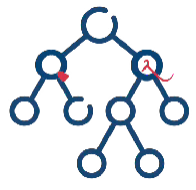
\includegraphics[height=0.9cm]{msca_logo.png}}%
  \end{center}
  \vspace{0.45cm}
  \begin{center}
    \begin{minipage}{0.1\textwidth}\centering
      \href{https://quantlet.com}{
\includegraphics[height=0.9cm]{ql_logo.png}}\end{minipage}%
    \begin{minipage}{0.78\textwidth}\centering
      {\Large\bfseries\usebeamercolor[fg]{title}\inserttitle}\par\vspace{0.25cm}
      {\large\usebeamercolor[fg]{title}\insertsubtitle}\end{minipage}%
    \begin{minipage}{0.1\textwidth}\centering
      \href{https://quantinar.com}{
\includegraphics[height=0.9cm]{qr_logo.png}}\end{minipage}
  \end{center}
  \vfill
  \hspace{0.4cm}{\bfseries\insertauthor}\par\vspace{0.12cm}
  \hspace{0.4cm}\begin{minipage}[t]{0.92\textwidth}\raggedright\footnotesize\insertinstitute\end{minipage}
  \par\vspace{0.4cm}}

% ---------------------------------------------------------------- lecture metadata
\newcommand{\nnshort}{}
\newcommand{\nnnb}{notebooks}
\newcommand{\nnrepo}{https://github.com/danpele/NEURAL_BIZ/tree/main}
% language-dependent labels (English default; \nnromanian switches to Romanian, call it before \nnlecture)
\newcommand{\txtcourse}{Neural Networks and Deep Learning}
\newcommand{\txtlecture}{Lecture}
\newcommand{\txtoutline}{Outline}
\newcommand{\txtintuition}{In one sentence:}
\newcommand{\txtjob}{In practice:}
\newcommand{\txttry}{Experiment yourself:}
\newcommand{\txtwhere}{where}
\newcommand{\txtsim}{SIMULATED DATA (teaching illustration)}
\newcommand{\txtnbsuffix}{}
\newcommand{\txtinstitute}{Bucharest University of Economic Studies (ASE), Department of Statistics and Econometrics\\
    Romanian Academy, Institute for Economic Forecasting (IPE)\\
    IDA Institute Digital Assets \textbullet\ AI4EFin \textbullet\ MSCA Digital Finance}
\newcommand{\nnromanian}{%
  \renewcommand{\txtcourse}{Rețele neuronale și deep learning}%
  \renewcommand{\txtlecture}{Cursul}%
  \renewcommand{\txtoutline}{Cuprins}%
  \renewcommand{\txtintuition}{Pe scurt:}%
  \renewcommand{\txtjob}{În practică:}%
  \renewcommand{\txttry}{Exercițiu practic:}%
  \renewcommand{\txtwhere}{unde}%
  \renewcommand{\txtsim}{DATE SIMULATE (doar pentru ilustrare)}%
  \renewcommand{\txtnbsuffix}{\string_ro}%
  \renewcommand{\txtinstitute}{Academia de Studii Economice din București (ASE), Departamentul de Statistică și Econometrie\\
    Academia Română, Institutul de Prognoză Economică (IPE)\\
    IDA Institute Digital Assets \textbullet\ AI4EFin \textbullet\ MSCA Digital Finance}}
\newcommand{\nnlecture}[2]{%
  \renewcommand{\nnshort}{\txtlecture\ #1}%
  \renewcommand{\nnnb}{notebooks/L#1\string_notebook\txtnbsuffix.ipynb}%
  \title[NN]{\txtcourse}%
  \subtitle{\txtlecture\ #1: #2}%
  \author{Prof.\ dr.\ Daniel Traian PELE}%
  \institute{\txtinstitute}%
  \date{}}

% ---------------------------------------------------------------- teaching blocks (one message per frame)
% \intuition{one plain sentence}  ->  formula with every symbol defined  ->  real-data example  ->  \manager{one line}
\newcommand{\intuition}[1]{\begin{itemize}\item {\color{MainBlue}\textbf{\txtintuition}}~#1\end{itemize}\vspace{0.6mm}}
\newcommand{\manager}[1]{\colorbox{Forest!10}{\parbox{\dimexpr\linewidth-2\fboxsep\relax}{\footnotesize
  \begin{itemize}\setlength{\itemsep}{0pt}\item \textbf{\color{Forest}\txtjob}~#1\end{itemize}}}}
% Experiment yourself: pointer to the matching notebook section
\newcommand{\tryit}[1]{{\scriptsize\href{\nnrepo/\nnnb}{%
  \raisebox{-0.15em}{
\includegraphics[height=0.85em]{ql_logo.png}}\,\textbf{\txttry}~\color{MainBlue}#1}}}
% bottom row: manager line (left) + experiment pointer (right), pinned to the bottom of the frame
\newcommand{\bottomrow}[2]{\par\vfill\noindent\begin{minipage}[b]{0.72\linewidth}#1\end{minipage}\hfill
  \begin{minipage}[b]{0.26\linewidth}\raggedleft #2\end{minipage}\par\vspace{0.5mm}}
\newcommand{\where}[1]{{\footnotesize\textbf{\txtwhere}~#1\par}}

% ---------------------------------------------------------------- helpers
% chart source line under a figure: \chartsource{Source ...; period ...}
\newcommand{\chartsource}[1]{\par\vspace{1pt}{\scriptsize\color{FooterGray}#1\par}}
% link to code: \quantlet{label}{path inside the repo}
\newcommand{\quantlet}[2]{\par\vspace{1pt}\hfill\href{\nnrepo/#2}{%
  \raisebox{-0.15em}{
\includegraphics[height=0.75em]{ql_logo.png}}\textcolor{MainBlue}{\scriptsize\ #1}}}
% inline Quantlet link for the bottom-right corner of a frame: \qlink{label}{path inside the repo}
\newcommand{\qlink}[2]{{\scriptsize\href{\nnrepo/#2}{\raisebox{-0.15em}{
\includegraphics[height=0.85em]{ql_logo.png}}\,\textcolor{MainBlue}{#1}}}}
\newcommand{\simlabel}{\colorbox{Crimson!12}{\scriptsize\bfseries\color{Crimson}\txtsim}}
\newcommand{\E}{\mathbb{E}}
\newcommand{\Var}{\operatorname{Var}}
\newcommand{\Cov}{\operatorname{Cov}}
\newcommand{\Corr}{\operatorname{Corr}}
\newcommand{\asinh}{\operatorname{asinh}}
\newcommand{\iid}{\overset{\text{i.i.d.}}{\sim}}
\newcommand{\EUR}{EUR}
% deep-learning notation (Bishop & Bishop, 2024): vectors bold lower case, matrices bold upper case
\newcommand{\R}{\mathbb{R}}
\newcommand{\vx}{\mathbf{x}}
\newcommand{\vy}{\mathbf{y}}
\newcommand{\vz}{\mathbf{z}}
\newcommand{\vh}{\mathbf{h}}
\newcommand{\vw}{\mathbf{w}}
\newcommand{\vb}{\mathbf{b}}
\newcommand{\mW}{\mathbf{W}}
\newcommand{\mX}{\mathbf{X}}
\newcommand{\btheta}{\boldsymbol{\theta}}
\newcommand{\loss}{\mathcal{L}}
\newcommand{\dataset}{\mathcal{D}}
\DeclareMathOperator*{\argmin}{arg\,min}
\DeclareMathOperator*{\argmax}{arg\,max}
\DeclareMathOperator{\softmax}{softmax}
\DeclareMathOperator{\ReLU}{ReLU}
\DeclareMathOperator{\sigm}{\sigma}

%   \nnlecture{k}{Lecture title}
% Logos live in lectures/common/logos/, charts in lectures/Lk/charts/.
% Do NOT add \hfuzz / \vfuzz / \hbadness here: overfull boxes must be fixed, not hidden.
% =============================================================================

\usetheme{default}
\setbeamersize{text margin left=7mm, text margin right=7mm}

% ---------------------------------------------------------------- packages
\usepackage[utf8]{inputenc}
\usepackage[T1]{fontenc}
\usepackage{lmodern}
\usepackage{amsmath, amssymb}
\usepackage{mathtools}
\usepackage{bm}
\usepackage{tikz}
\usetikzlibrary{arrows.meta, positioning, calc, shapes.misc}
\usepackage{booktabs}
\usepackage{array}
\usepackage{graphicx}
\usepackage{colortbl}
\usepackage{xcolor}
\usepackage{multicol}
\hypersetup{colorlinks=true, linkcolor=MainBlue, urlcolor=MainBlue, citecolor=MainBlue}
\graphicspath{{../common/logos/}}   % charts are included with their language folder: charts/en/, charts/ro/

% ---------------------------------------------------------------- colours
\definecolor{MainBlue}{RGB}{26, 58, 110}
\definecolor{IDAred}{RGB}{205, 0, 0}
\definecolor{DarkGray}{RGB}{51, 51, 51}
\definecolor{FooterGray}{RGB}{100, 100, 100}
\definecolor{BlockGray}{RGB}{236, 238, 242}
\definecolor{KeynoteGray}{RGB}{218, 218, 218}
\definecolor{Crimson}{RGB}{190, 40, 50}
\definecolor{Forest}{RGB}{30, 110, 50}
\definecolor{Bitter}{RGB}{214, 150, 20}
% chart palette (same hex values and order as lectures/common/nn_plot.py SERIES)
\definecolor{Ser1}{HTML}{2A78D6}
\definecolor{Ser2}{HTML}{EB6834}
\definecolor{Ser3}{HTML}{1BAF7A}
\definecolor{Ser4}{HTML}{EDA100}
\definecolor{Ser5}{HTML}{E87BA4}
\definecolor{Ser6}{HTML}{008300}
\definecolor{Ser7}{HTML}{6250D6}
\definecolor{Ser8}{HTML}{E34948}

\setbeamertemplate{background}{%
  \begin{tikzpicture}[remember picture, overlay]
    \shade[shading=axis, shading angle=315, top color=white, bottom color=KeynoteGray]
      (current page.south west) rectangle (current page.north east);
  \end{tikzpicture}}
\setbeamercolor{background canvas}{bg=}
\setbeamercolor{structure}{fg=MainBlue}
\setbeamercolor{normal text}{fg=DarkGray}
\setbeamercolor{title}{fg=IDAred}
\setbeamercolor{frametitle}{fg=IDAred, bg=}
\setbeamercolor{block title}{bg=MainBlue, fg=white}
\setbeamercolor{block body}{bg=BlockGray, fg=DarkGray}
\setbeamercolor{block title alerted}{bg=Crimson, fg=white}
\setbeamercolor{block body alerted}{bg=Crimson!7, fg=DarkGray}
\setbeamercolor{block title example}{bg=Forest, fg=white}
\setbeamercolor{block body example}{bg=Forest!7, fg=DarkGray}
\setbeamercolor{item}{fg=MainBlue}
\setbeamerfont{frametitle}{size=\large, series=\bfseries}
\setbeamerfont{block title}{size=\small, series=\bfseries}
\setbeamertemplate{blocks}[rounded][shadow=false]
\setbeamertemplate{itemize item}{\color{MainBlue}$\boxdot$}
\setbeamertemplate{itemize subitem}{\color{MainBlue}\scriptsize$\blacktriangleright$}
% compact two-level lists: level 1 = main point, level 2 = details (no text outside bullets)
\setbeamerfont{itemize/enumerate subbody}{size=\footnotesize}
\setlength{\leftmargini}{1.1em}
\setlength{\leftmarginii}{1.1em}
\setbeamertemplate{itemize/enumerate body begin}{\setlength{\topsep}{0pt}\setlength{\partopsep}{0pt}\setlength{\parskip}{0pt}}
\setbeamertemplate{itemize/enumerate subbody begin}{\setlength{\topsep}{0pt}\setlength{\partopsep}{0pt}\setlength{\itemsep}{0pt}\vspace{-0.4ex}}

\setbeamertemplate{enumerate item}{\color{MainBlue}\insertenumlabel.}
\setlength{\leftmargini}{1.3em}
\setlength{\leftmarginii}{1.2em}
\setbeamertemplate{navigation symbols}{}
\setbeamertemplate{section in toc}{\color{MainBlue}$\blacktriangleright$~\inserttocsection}
\setbeamertemplate{caption}{\raggedright\insertcaption\par}
% frame subtitle = precise citation line under the claim title (Weron style)
\setbeamerfont{framesubtitle}{size=\footnotesize}
\setbeamercolor{framesubtitle}{fg=FooterGray}
% outline that reappears at every section with the current section highlighted
\setbeamertemplate{section in toc shaded}[default][35]
\setbeamertemplate{subsection in toc shaded}[default][35]
\setbeamertemplate{subsection in toc}{\leavevmode\leftskip=2.2em\color{DarkGray}\small\inserttocsubsection\par}
\AtBeginSection[]{{\begin{frame}{\txtoutline}\vspace{2mm}\small
  \tableofcontents[currentsection,hideothersubsections]\end{frame}}}

% ---------------------------------------------------------------- head and foot
\setbeamertemplate{headline}{%
  \vskip10pt%
  \hbox to \paperwidth{\hskip0.5cm%
    {\small\color{FooterGray}\renewcommand{\hyperlink}[2]{##2}\insertsectionhead}%
    \hfill\textcolor{FooterGray}{\small\insertframenumber}\hskip0.5cm}%
  \vskip4pt{\color{FooterGray}\hrule height 0.4pt}}
% footer as in the other courses (MFM, SFM): course name on the left, small sparkline on the right
\setbeamertemplate{footline}{%
  {\color{FooterGray}\hrule height 0.4pt}\vskip4pt%
  \hbox to \paperwidth{\hskip0.5cm%
    \textcolor{FooterGray}{\small\txtcourse}%
    \hfill\raisebox{-0.1em}{\begin{tikzpicture}[x=0.08em, y=0.08em, line width=0.4pt]
      \draw[FooterGray] (0,3) -- (1,4) -- (2,3.5) -- (3,5) -- (4,4) -- (5,6) -- (6,5.5) -- (7,4) -- (8,5) -- (9,7) -- (10,6) -- (11,5) -- (12,6.5) -- (13,8) -- (14,7) -- (15,6) -- (16,7.5) -- (17,9) -- (18,8) -- (19,7) -- (20,8.5) -- (21,10) -- (22,9) -- (23,8) -- (24,9.5);
    \end{tikzpicture}}\hskip0.5cm}%
  \vskip6pt}

% ---------------------------------------------------------------- title page
\defbeamertemplate*{title page}{nn}[1][]{%
  \vspace{0.15cm}
  \begin{center}
    \href{https://www.ase.ro}{
\includegraphics[height=0.9cm]{ase_logo.png}}\hspace{0.3cm}%
    \href{https://ipe.ro/new}{
\includegraphics[height=0.9cm]{acad_logo.png}}\hspace{0.3cm}%
    \href{https://theida.net}{
\includegraphics[height=0.9cm]{ida_logo.png}}\hspace{0.3cm}%
    \href{https://blockchain-research-center.com}{
\includegraphics[height=0.9cm]{brc_logo.png}}\hspace{0.3cm}%
    \href{https://www.ai4efin.ase.ro}{
\includegraphics[height=0.9cm]{ai4efin_logo.png}}\hspace{0.3cm}%
    \href{https://www.digital-finance-msca.com}{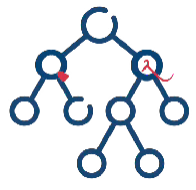
\includegraphics[height=0.9cm]{msca_logo.png}}%
  \end{center}
  \vspace{0.45cm}
  \begin{center}
    \begin{minipage}{0.1\textwidth}\centering
      \href{https://quantlet.com}{
\includegraphics[height=0.9cm]{ql_logo.png}}\end{minipage}%
    \begin{minipage}{0.78\textwidth}\centering
      {\Large\bfseries\usebeamercolor[fg]{title}\inserttitle}\par\vspace{0.25cm}
      {\large\usebeamercolor[fg]{title}\insertsubtitle}\end{minipage}%
    \begin{minipage}{0.1\textwidth}\centering
      \href{https://quantinar.com}{
\includegraphics[height=0.9cm]{qr_logo.png}}\end{minipage}
  \end{center}
  \vfill
  \hspace{0.4cm}{\bfseries\insertauthor}\par\vspace{0.12cm}
  \hspace{0.4cm}\begin{minipage}[t]{0.92\textwidth}\raggedright\footnotesize\insertinstitute\end{minipage}
  \par\vspace{0.4cm}}

% ---------------------------------------------------------------- lecture metadata
\newcommand{\nnshort}{}
\newcommand{\nnnb}{notebooks}
\newcommand{\nnrepo}{https://github.com/danpele/NEURAL_BIZ/tree/main}
% language-dependent labels (English default; \nnromanian switches to Romanian, call it before \nnlecture)
\newcommand{\txtcourse}{Neural Networks and Deep Learning}
\newcommand{\txtlecture}{Lecture}
\newcommand{\txtoutline}{Outline}
\newcommand{\txtintuition}{In one sentence:}
\newcommand{\txtjob}{In practice:}
\newcommand{\txttry}{Experiment yourself:}
\newcommand{\txtwhere}{where}
\newcommand{\txtsim}{SIMULATED DATA (teaching illustration)}
\newcommand{\txtnbsuffix}{}
\newcommand{\txtinstitute}{Bucharest University of Economic Studies (ASE), Department of Statistics and Econometrics\\
    Romanian Academy, Institute for Economic Forecasting (IPE)\\
    IDA Institute Digital Assets \textbullet\ AI4EFin \textbullet\ MSCA Digital Finance}
\newcommand{\nnromanian}{%
  \renewcommand{\txtcourse}{Rețele neuronale și deep learning}%
  \renewcommand{\txtlecture}{Cursul}%
  \renewcommand{\txtoutline}{Cuprins}%
  \renewcommand{\txtintuition}{Pe scurt:}%
  \renewcommand{\txtjob}{În practică:}%
  \renewcommand{\txttry}{Exercițiu practic:}%
  \renewcommand{\txtwhere}{unde}%
  \renewcommand{\txtsim}{DATE SIMULATE (doar pentru ilustrare)}%
  \renewcommand{\txtnbsuffix}{\string_ro}%
  \renewcommand{\txtinstitute}{Academia de Studii Economice din București (ASE), Departamentul de Statistică și Econometrie\\
    Academia Română, Institutul de Prognoză Economică (IPE)\\
    IDA Institute Digital Assets \textbullet\ AI4EFin \textbullet\ MSCA Digital Finance}}
\newcommand{\nnlecture}[2]{%
  \renewcommand{\nnshort}{\txtlecture\ #1}%
  \renewcommand{\nnnb}{notebooks/L#1\string_notebook\txtnbsuffix.ipynb}%
  \title[NN]{\txtcourse}%
  \subtitle{\txtlecture\ #1: #2}%
  \author{Prof.\ dr.\ Daniel Traian PELE}%
  \institute{\txtinstitute}%
  \date{}}

% ---------------------------------------------------------------- teaching blocks (one message per frame)
% \intuition{one plain sentence}  ->  formula with every symbol defined  ->  real-data example  ->  \manager{one line}
\newcommand{\intuition}[1]{\begin{itemize}\item {\color{MainBlue}\textbf{\txtintuition}}~#1\end{itemize}\vspace{0.6mm}}
\newcommand{\manager}[1]{\colorbox{Forest!10}{\parbox{\dimexpr\linewidth-2\fboxsep\relax}{\footnotesize
  \begin{itemize}\setlength{\itemsep}{0pt}\item \textbf{\color{Forest}\txtjob}~#1\end{itemize}}}}
% Experiment yourself: pointer to the matching notebook section
\newcommand{\tryit}[1]{{\scriptsize\href{\nnrepo/\nnnb}{%
  \raisebox{-0.15em}{
\includegraphics[height=0.85em]{ql_logo.png}}\,\textbf{\txttry}~\color{MainBlue}#1}}}
% bottom row: manager line (left) + experiment pointer (right), pinned to the bottom of the frame
\newcommand{\bottomrow}[2]{\par\vfill\noindent\begin{minipage}[b]{0.72\linewidth}#1\end{minipage}\hfill
  \begin{minipage}[b]{0.26\linewidth}\raggedleft #2\end{minipage}\par\vspace{0.5mm}}
\newcommand{\where}[1]{{\footnotesize\textbf{\txtwhere}~#1\par}}

% ---------------------------------------------------------------- helpers
% chart source line under a figure: \chartsource{Source ...; period ...}
\newcommand{\chartsource}[1]{\par\vspace{1pt}{\scriptsize\color{FooterGray}#1\par}}
% link to code: \quantlet{label}{path inside the repo}
\newcommand{\quantlet}[2]{\par\vspace{1pt}\hfill\href{\nnrepo/#2}{%
  \raisebox{-0.15em}{
\includegraphics[height=0.75em]{ql_logo.png}}\textcolor{MainBlue}{\scriptsize\ #1}}}
% inline Quantlet link for the bottom-right corner of a frame: \qlink{label}{path inside the repo}
\newcommand{\qlink}[2]{{\scriptsize\href{\nnrepo/#2}{\raisebox{-0.15em}{
\includegraphics[height=0.85em]{ql_logo.png}}\,\textcolor{MainBlue}{#1}}}}
\newcommand{\simlabel}{\colorbox{Crimson!12}{\scriptsize\bfseries\color{Crimson}\txtsim}}
\newcommand{\E}{\mathbb{E}}
\newcommand{\Var}{\operatorname{Var}}
\newcommand{\Cov}{\operatorname{Cov}}
\newcommand{\Corr}{\operatorname{Corr}}
\newcommand{\asinh}{\operatorname{asinh}}
\newcommand{\iid}{\overset{\text{i.i.d.}}{\sim}}
\newcommand{\EUR}{EUR}
% deep-learning notation (Bishop & Bishop, 2024): vectors bold lower case, matrices bold upper case
\newcommand{\R}{\mathbb{R}}
\newcommand{\vx}{\mathbf{x}}
\newcommand{\vy}{\mathbf{y}}
\newcommand{\vz}{\mathbf{z}}
\newcommand{\vh}{\mathbf{h}}
\newcommand{\vw}{\mathbf{w}}
\newcommand{\vb}{\mathbf{b}}
\newcommand{\mW}{\mathbf{W}}
\newcommand{\mX}{\mathbf{X}}
\newcommand{\btheta}{\boldsymbol{\theta}}
\newcommand{\loss}{\mathcal{L}}
\newcommand{\dataset}{\mathcal{D}}
\DeclareMathOperator*{\argmin}{arg\,min}
\DeclareMathOperator*{\argmax}{arg\,max}
\DeclareMathOperator{\softmax}{softmax}
\DeclareMathOperator{\ReLU}{ReLU}
\DeclareMathOperator{\sigm}{\sigma}

\nnlecture{9}{Graph neural networks}
\begin{document}
{\setbeamertemplate{headline}{}\setbeamertemplate{footline}{}
\begin{frame}\titlepage\end{frame}}
% END-FRONT-MATTER

\begin{frame}{Learning objectives}
\small
\begin{itemize}\setlength{\itemsep}{5pt}
  \item Represent financial data as a graph: nodes, edges, node features
    \begin{itemize}\setlength{\itemsep}{0pt}
      \item Adjacency, degree and the normalised adjacency matrix.
    \end{itemize}
  \item Write the message-passing scheme of a graph neural network (GNN) and its three classic layers: graph convolutional network (GCN), graph sample and aggregate (GraphSAGE), graph attention network (GAT).
  \item Train them on the Elliptic Bitcoin graph for anti-money laundering (AML), in time order, against a logistic regression and a random forest.
  \item Judge the results like an investigator: precision, recall, the area under the precision-recall curve (PR-AUC), alerts per analyst, drift and stability of explanations.
\end{itemize}
\end{frame}

% BEGIN-ABBR

\begin{frame}{Abbreviations}
\small
\vspace{-1mm}\begin{columns}[T,onlytextwidth]
\begin{column}{0.49\textwidth}{\scriptsize\renewcommand{\arraystretch}{0.96}\begin{tabular}{@{}>{\bfseries}l@{\ \ }p{0.74\linewidth}@{}}AML & anti-money laundering\\
ASE & Bucharest University of Economic Studies\\
BTC & bitcoin (currency unit)\\
CNN & convolutional neural network\\
CPU & central processing unit\\
GAT & graph attention network\\
GCN & graph convolutional network\\
GIN & graph isomorphism network\\
GNN & graph neural network\\
GraphSAGE & graph sample and aggregate\\\end{tabular}}\end{column}
\begin{column}{0.49\textwidth}{\scriptsize\renewcommand{\arraystretch}{0.96}\begin{tabular}{@{}>{\bfseries}l@{\ \ }p{0.74\linewidth}@{}}IPE & Institute for Economic Forecasting, Romanian Academy\\
MLP & multilayer perceptron\\
MPNN & message-passing neural network\\
PCA & principal component analysis\\
PR-AUC & area under the precision-recall curve\\
PyG & PyTorch Geometric (library)\\
ReLU & rectified linear unit\\
SHAP & SHapley Additive exPlanations\\
WL & Weisfeiler--Leman graph isomorphism test\\
XAI & explainable artificial intelligence\\\end{tabular}}\end{column}
\end{columns}
\end{frame}

% END-ABBR


\section{Why graphs for financial crime}

\begin{frame}{Money laundering hides in the links, not in the rows}
\footnotesize
\intuition{A single payment can look ordinary; the chain of payments around it often does not.}
\begin{columns}[T,onlytextwidth]
\begin{column}{0.53\textwidth}
\[ G=(\mathcal V,\mathcal E,\mathbf X),\qquad \mathbf X\in\R^{n\times d},\qquad y_v\in\{0,1\} \]{\footnotesize\begin{itemize}\setlength{\itemsep}{0pt}
  \item \textbf{\txtwhere}
    \begin{itemize}\setlength{\itemsep}{0pt}
      \item $\mathcal V$ = nodes (transactions), $n=|\mathcal V|$
      \item $\mathcal E$ = edges (a payment flow from one transaction to the next)
      \item $\mathbf X$ = node features, $d$ per node
      \item $y_v=1$ if transaction $v$ is illicit.
    \end{itemize}
\end{itemize}\par}
\end{column}
\begin{column}{0.44\textwidth}
\begin{itemize}\setlength{\itemsep}{3pt}
  \item \textbf{Elliptic graph} (Weber et al., 2019)
    \begin{itemize}\setlength{\itemsep}{0pt}
      \item 203\,769 Bitcoin transactions, 234\,355 payment flows
      \item 165 features per transaction, 49 time steps
    \end{itemize}
  \item \textbf{The task}
    \begin{itemize}\setlength{\itemsep}{0pt}
      \item Node classification: illicit (scams, ransomware, dark markets) or licit
    \end{itemize}
\end{itemize}
\end{column}
\end{columns}
\par\vfill\manager{a bank's anti-money-laundering team already thinks in chains of payments
    \begin{itemize}\setlength{\itemsep}{0pt}
      \item A GNN learns from the same chains.
    \end{itemize}}\par\vspace{0.5mm}
\par\vfill\noindent{\scriptsize\color{FooterGray}(Weber et al., 2019; Bishop \& Bishop, 2024, ch.\ 13)}\hfill\tryit{notebook \S1}\par\vspace{0.5mm}
\end{frame}

\begin{frame}{The Elliptic data in one table}
\footnotesize
{\scriptsize\renewcommand{\arraystretch}{1.05}\setlength{\tabcolsep}{4pt}
\begin{tabular}{@{}p{0.30\textwidth}p{0.62\textwidth}@{}}\toprule
Element & Value in our copy of the data \\ \midrule
Nodes, edges & 203\,769 transactions; 234\,355 directed payment flows \\
Labels & 4\,545 illicit, 42\,019 licit, 157\,205 unknown (22.9\,\% labelled) \\
Features & 93 local (amounts, fees, inputs, outputs) + 72 aggregated over the neighbours \\
Time & 49 steps of about two weeks; edges join transactions of the same step (100.0\,\%) \\
Training / test & steps 1--34 (29\,894 labelled) / steps 35--49 (16\,670 labelled, 1\,083 illicit) \\
\bottomrule\end{tabular}}
\vspace{1mm}
\begin{itemize}\setlength{\itemsep}{2pt}
  \item \textbf{Imbalance}: only 9.76\,\% of the labelled transactions are illicit
    \begin{itemize}\setlength{\itemsep}{0pt}
      \item Accuracy alone would be meaningless.
    \end{itemize}
  \item \textbf{Anonymised}: the feature names are hidden by Elliptic
    \begin{itemize}\setlength{\itemsep}{0pt}
      \item We read them as $f_1,\dots,f_{165}$.
    \end{itemize}
\end{itemize}
\par\vfill\noindent{\scriptsize\color{FooterGray}(Weber et al., 2019)}\hfill\tryit{notebook \S1}\par\vspace{0.5mm}
\end{frame}

\begin{frame}{Labels arrive in waves: illicit activity is not stationary}
\small
\begin{center}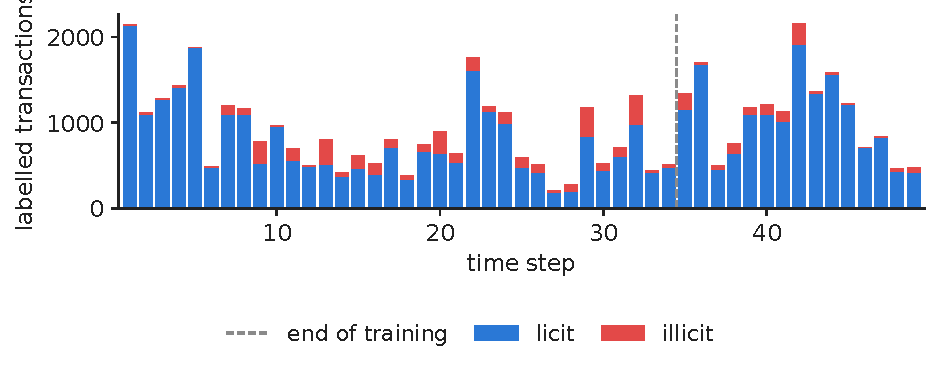
\includegraphics[width=\textwidth,height=0.441\textheight,keepaspectratio]{charts/en/elliptic_timesteps.pdf}\end{center}\vspace{-3mm}
\chartsource{Source: Elliptic Bitcoin transaction graph (Weber et al., 2019). Data: Elliptic Bitcoin transaction graph, 49 time steps (about two weeks each).}
\vspace{0.5mm}
\begin{itemize}\setlength{\itemsep}{0pt}
  \item \textbf{Peak}: 342 illicit transactions in step 32
    \begin{itemize}\setlength{\itemsep}{0pt}
      \item About 4\,159 transactions per step in total.
    \end{itemize}
  \item \textbf{Split in time}: train on steps 1--34, test once on steps 35--49, as in Weber et al.\ (2019)
    \begin{itemize}\setlength{\itemsep}{0pt}
      \item Never shuffle the steps.
    \end{itemize}
\end{itemize}
\par\vfill\manager{a model is judged on the months after its training data, exactly as it will be used.}\par\vspace{0.5mm}
\par\vfill\noindent{\scriptsize\color{FooterGray}}\hfill\qlink{NN\_L9\_elliptic\_timesteps}{Quantlets/L9/NN_L9_elliptic_timesteps}\par\vspace{0.5mm}
\end{frame}

\begin{frame}{Most transactions touch one or two others; a few are hubs}
\small
\begin{center}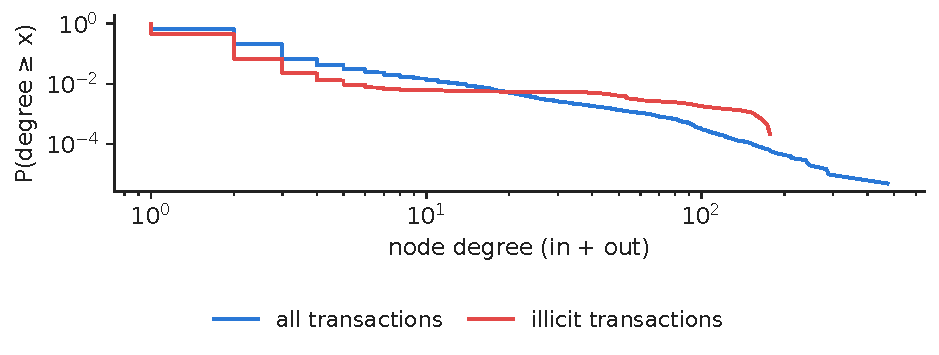
\includegraphics[width=\textwidth,height=0.519\textheight,keepaspectratio]{charts/en/degree_dist.pdf}\end{center}\vspace{-3mm}
\chartsource{Source: Elliptic Bitcoin transaction graph (Weber et al., 2019). Data: Elliptic Bitcoin transaction graph, 49 time steps (about two weeks each).}
\vspace{0.5mm}
\begin{itemize}\setlength{\itemsep}{0pt}
  \item \textbf{Sparse graph}: mean degree 2.30, median 2
    \begin{itemize}\setlength{\itemsep}{0pt}
      \item 34.5\,\% of the nodes have one neighbour only.
    \end{itemize}
  \item \textbf{Heavy tail}: the largest hub has 473 neighbours
    \begin{itemize}\setlength{\itemsep}{0pt}
      \item A GNN must not let hubs drown everyone else (hence the normalisation).
    \end{itemize}
\end{itemize}
\par\vfill\noindent{\scriptsize\color{FooterGray}$\deg(v)=|\mathcal N(v)|$}\hfill\qlink{NN\_L9\_degree\_dist}{Quantlets/L9/NN_L9_degree_dist}\par\vspace{0.5mm}
\end{frame}

\begin{frame}{Illicit transactions sit next to illicit transactions}
\small
\begin{center}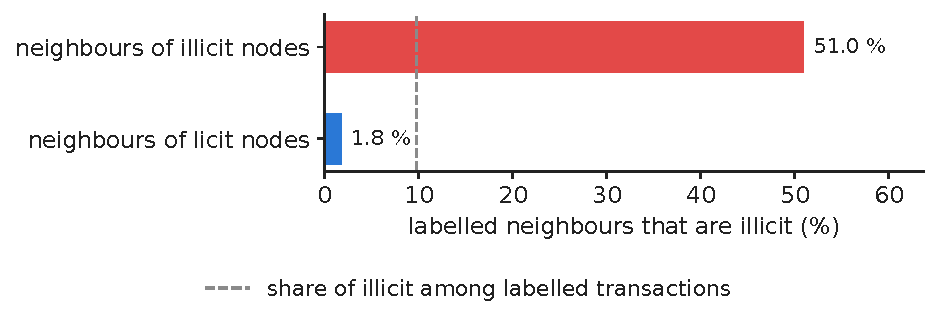
\includegraphics[width=\textwidth,height=0.480\textheight,keepaspectratio]{charts/en/homophily.pdf}\end{center}\vspace{-3mm}
\chartsource{Source: Elliptic Bitcoin transaction graph (Weber et al., 2019). Data: Elliptic Bitcoin transaction graph, 49 time steps (about two weeks each).}
\vspace{0.5mm}
\begin{itemize}\setlength{\itemsep}{0pt}
  \item \textbf{Homophily}: 51.0\,\% of the labelled neighbours of an illicit node are illicit, against 1.8\,\% for a licit node.
  \item \textbf{Edge homophily} 95.4\,\% of the labelled edges join the same class
    \begin{itemize}\setlength{\itemsep}{0pt}
      \item With random labels: 82.4\,\%.
    \end{itemize}
\end{itemize}
\par\vfill\manager{homophily is the reason to look at the neighbours: who you trade with says something about you.}\par\vspace{0.5mm}
\par\vfill\noindent{\scriptsize\color{FooterGray}}\hfill\qlink{NN\_L9\_homophily}{Quantlets/L9/NN_L9_homophily}\par\vspace{0.5mm}
\end{frame}


\section{Graphs as matrices}

\begin{frame}{The adjacency matrix turns a graph into linear algebra}
\footnotesize
\intuition{Every operation of a GNN is a product of the feature matrix with a (normalised) adjacency matrix and a weight matrix.}
\begin{columns}[T,onlytextwidth]
\begin{column}{0.53\textwidth}
\[ A_{uv}=\begin{cases}1,&(u,v)\in\mathcal E\\0,&\text{otherwise}\end{cases},\qquad D=\operatorname{diag}\Big(\sum_v A_{uv}\Big) \]\[ \tilde A=A+I,\qquad \hat A=\tilde D^{-1/2}\tilde A\,\tilde D^{-1/2} \]{\footnotesize\begin{itemize}\setlength{\itemsep}{0pt}
  \item \textbf{\txtwhere}
    \begin{itemize}\setlength{\itemsep}{0pt}
      \item $A$ = adjacency, symmetrised
      \item $D$ = degree matrix
      \item $\tilde A$ adds self-loops (a node keeps its own features)
      \item $\hat A$ has entries $1/\sqrt{\tilde d_u\tilde d_v}$.
    \end{itemize}
\end{itemize}\par}
\end{column}
\begin{column}{0.44\textwidth}
\begin{itemize}\setlength{\itemsep}{3pt}
  \item \textbf{Sparse storage}
    \begin{itemize}\setlength{\itemsep}{0pt}
      \item $A$ has $n^2\approx 4\cdot 10^{10}$ cells but only 234\,355 edges
      \item Libraries keep an edge list $2\times|\mathcal E|$, as in PyTorch Geometric (PyG)
    \end{itemize}
  \item \textbf{Why normalise}
    \begin{itemize}\setlength{\itemsep}{0pt}
      \item Without it a hub of degree 473 would add 473 messages and explode the scale
    \end{itemize}
\end{itemize}
\end{column}
\end{columns}
\par\vfill\manager{a bank's payment network is stored as an edge list, never as a dense matrix.}\par\vspace{0.5mm}
\par\vfill\noindent{\scriptsize\color{FooterGray}(Kipf \& Welling, 2017)}\hfill\tryit{notebook \S2}\par\vspace{0.5mm}
\end{frame}

\begin{frame}{A graph model must not depend on how we number the nodes}
\footnotesize
\intuition{Transaction 17 and transaction 4,203 are names, not positions; relabelling them must not change any prediction.}
\begin{columns}[T,onlytextwidth]
\begin{column}{0.53\textwidth}
\[ f\big(P\mathbf X,\;PAP^{\top}\big)=P\,f(\mathbf X,A)\quad\forall P \]{\footnotesize\begin{itemize}\setlength{\itemsep}{0pt}
  \item \textbf{\txtwhere}
    \begin{itemize}\setlength{\itemsep}{0pt}
      \item $P$ = any $n\times n$ permutation matrix
      \item $f$ returns one output row per node: \textit{equivariance}
      \item A graph-level output must be \textit{invariant}: $g(P\mathbf X,PAP^{\top})=g(\mathbf X,A)$.
    \end{itemize}
\end{itemize}\par}
\end{column}
\begin{column}{0.44\textwidth}
\begin{itemize}\setlength{\itemsep}{3pt}
  \item \textbf{Why not a multilayer perceptron (MLP)?}
    \begin{itemize}\setlength{\itemsep}{0pt}
      \item On the rows of $A$ it would need $n$ inputs and change with the numbering
    \end{itemize}
  \item \textbf{Why not a convolutional neural network (CNN)?}
    \begin{itemize}\setlength{\itemsep}{0pt}
      \item It assumes a grid with a fixed number of ordered neighbours
      \item A node has between 1 and 473 neighbours, in no order
    \end{itemize}
\end{itemize}
\end{column}
\end{columns}
\par\vfill\manager{ask of any vendor model: does the score change if the input file is sorted differently? It must not.}\par\vspace{0.5mm}
\par\vfill\noindent{\scriptsize\color{FooterGray}(Bishop \& Bishop, 2024, sec.\ 13.1)}\par\vspace{0.5mm}
\end{frame}

\begin{frame}{Smooth signals on a graph: the Laplacian}
\footnotesize
\intuition{The graph Laplacian measures how much a node signal differs between neighbours; GCN layers are low-pass filters of it.}
\begin{columns}[T,onlytextwidth]
\begin{column}{0.53\textwidth}
\[ L=D-A,\qquad \mathbf x^{\top}L\,\mathbf x=\sum_{(u,v)\in\mathcal E}\big(x_u-x_v\big)^2\ \ge 0 \]\[ L=U\Lambda U^{\top},\qquad \hat{\mathbf x}=U^{\top}\mathbf x\ \ (\text{graph Fourier transform}) \]{\footnotesize\begin{itemize}\setlength{\itemsep}{0pt}
  \item \textbf{\txtwhere}
    \begin{itemize}\setlength{\itemsep}{0pt}
      \item $\mathbf x\in\R^n$ = one feature on all nodes
      \item Small $\mathbf x^{\top}L\mathbf x$ = neighbours look alike (homophily)
      \item $U$, $\Lambda$ = eigenvectors and eigenvalues of $L$ (frequencies).
    \end{itemize}
\end{itemize}\par}
\end{column}
\begin{column}{0.44\textwidth}
\begin{itemize}\setlength{\itemsep}{3pt}
  \item \textbf{Spectral filter}
    \begin{itemize}\setlength{\itemsep}{0pt}
      \item $g_\theta\star\mathbf x=U\,g_\theta(\Lambda)\,U^{\top}\mathbf x$
      \item Costly: $U$ is dense, $O(n^2)$
    \end{itemize}
  \item \textbf{GCN}
    \begin{itemize}\setlength{\itemsep}{0pt}
      \item First-order polynomial in $L$ gives $\hat A$ of the previous slide
      \item Derivation in Appendix A
    \end{itemize}
\end{itemize}
\end{column}
\end{columns}
\par\vfill\manager{homophilous fraud graphs are smooth signals: averaging over neighbours removes noise, not information.}\par\vspace{0.5mm}
\par\vfill\noindent{\scriptsize\color{FooterGray}(Kipf \& Welling, 2017; Hamilton, 2020, ch.\ 7)}\par\vspace{0.5mm}
\end{frame}

\begin{frame}{Node, edge or graph: three prediction tasks}
\footnotesize
\intuition{The same message-passing layers serve three kinds of business questions; only the read-out changes.}
\begin{columns}[T,onlytextwidth]
\begin{column}{0.53\textwidth}
\[ \hat y_v=\sigma(\mathbf w^{\top}\mathbf h_v),\quad \hat y_{uv}=\sigma(\mathbf h_u^{\top}\mathbf h_v),\quad \hat y_G=\sigma\Big(\mathbf w^{\top}\sum_{v}\mathbf h_v\Big) \]{\footnotesize\begin{itemize}\setlength{\itemsep}{0pt}
  \item \textbf{\txtwhere}
    \begin{itemize}\setlength{\itemsep}{0pt}
      \item $\mathbf h_v$ = representation of node $v$ after the last layer
      \item $\sigma$ = logistic function
      \item The sum makes the graph output permutation-invariant.
    \end{itemize}
\end{itemize}\par}
\end{column}
\begin{column}{0.44\textwidth}
\begin{itemize}\setlength{\itemsep}{3pt}
  \item \textbf{Node}
    \begin{itemize}\setlength{\itemsep}{0pt}
      \item Is this transaction illicit? (this lecture)
    \end{itemize}
  \item \textbf{Edge}
    \begin{itemize}\setlength{\itemsep}{0pt}
      \item Will these two firms trade; is this payment a mule transfer?
    \end{itemize}
  \item \textbf{Graph}
    \begin{itemize}\setlength{\itemsep}{0pt}
      \item Is this cluster of accounts a laundering ring; is this interbank network fragile?
    \end{itemize}
\end{itemize}
\end{column}
\end{columns}
\par\vfill\manager{define the unit of decision first (a payment, a client, a ring), then the graph task.}\par\vspace{0.5mm}
\par\vfill\noindent{\scriptsize\color{FooterGray}(Hamilton, 2020, ch.\ 1)}\par\vspace{0.5mm}
\end{frame}


\section{Message passing}

\begin{frame}{A GNN layer: collect messages, aggregate, update}
\footnotesize
\intuition{Each node sends a message to its neighbours; each node sums what it receives and updates its own state.}
\begin{columns}[T,onlytextwidth]
\begin{column}{0.56\textwidth}
\[ \mathbf m_v^{(l)}=\bigoplus_{u\in\mathcal N(v)}\phi^{(l)}\big(\mathbf h_u^{(l)},\mathbf h_v^{(l)},\mathbf e_{uv}\big) \]\[ \mathbf h_v^{(l+1)}=\psi^{(l)}\big(\mathbf h_v^{(l)},\mathbf m_v^{(l)}\big),\qquad \mathbf h_v^{(0)}=\mathbf x_v \]{\footnotesize\begin{itemize}\setlength{\itemsep}{0pt}
  \item \textbf{\txtwhere}
    \begin{itemize}\setlength{\itemsep}{0pt}
      \item $\mathcal N(v)$ = neighbours of $v$
      \item $\phi$ = message function
      \item $\bigoplus$ = permutation-invariant aggregator (sum, mean, max)
      \item $\psi$ = update (a small network)
      \item $\mathbf e_{uv}$ = edge features, if any.
    \end{itemize}
\end{itemize}\par}
\end{column}
\begin{column}{0.41\textwidth}
\begin{center}\begin{tikzpicture}[scale=0.9, every node/.style={circle, draw=MainBlue, thick, minimum size=6mm, inner sep=0pt, font=\scriptsize}]
\node[fill=Ser2!35] (v) at (0,0) {$v$};
\node (a) at (-1.6,0.9) {$u_1$};
\node[fill=Ser8!30] (b) at (-1.7,-0.8) {$u_2$};
\node (c) at (1.6,0.9) {$u_3$};
\node (d) at (2.9,0.2) {$w$};
\draw[-{Stealth}, thick, Ser1] (a) -- node[draw=none, above, font=\tiny] {$\mathbf m_{u_1v}$} (v);
\draw[-{Stealth}, thick, Ser1] (b) -- (v);
\draw[-{Stealth}, thick, Ser1] (c) -- (v);
\draw[thick, FooterGray] (c) -- (d);
\end{tikzpicture}\end{center}\begin{itemize}\setlength{\itemsep}{2pt}
  \item \textbf{Message-passing neural network (MPNN)}: every layer of this lecture is a choice of $\phi$, $\bigoplus$, $\psi$.
\end{itemize}
\end{column}
\end{columns}
\par\vfill\manager{the weights $\phi,\psi$ are shared by all nodes: the model size does not grow with the graph.}\par\vspace{0.5mm}
\par\vfill\noindent{\scriptsize\color{FooterGray}(Gilmer et al., 2017; Bishop \& Bishop, 2024, sec.\ 13.2)}\hfill\tryit{notebook \S3}\par\vspace{0.5mm}
\end{frame}

\begin{frame}{The aggregator decides what a GNN can tell apart}
\footnotesize
\intuition{Mean and max forget how many neighbours sent a message; the sum keeps it, which makes it as powerful as the Weisfeiler--Leman test.}
\begin{columns}[T,onlytextwidth]
\begin{column}{0.53\textwidth}
\[ \mathbf h_v^{(l+1)}=\text{MLP}^{(l)}\Big((1+\varepsilon)\,\mathbf h_v^{(l)}+\sum_{u\in\mathcal N(v)}\mathbf h_u^{(l)}\Big) \]{\footnotesize\begin{itemize}\setlength{\itemsep}{0pt}
  \item \textbf{\txtwhere}
    \begin{itemize}\setlength{\itemsep}{0pt}
      \item Graph isomorphism network (GIN) layer
      \item $\varepsilon$ = learnable scalar
      \item A sum over a multiset is injective if the MLP is rich enough, so GIN separates any two neighbourhoods that the Weisfeiler--Leman (WL) test separates.
    \end{itemize}
\end{itemize}\par}
\end{column}
\begin{column}{0.44\textwidth}
\begin{itemize}\setlength{\itemsep}{3pt}
  \item \textbf{Example}
    \begin{itemize}\setlength{\itemsep}{0pt}
      \item Neighbours $\{a,a\}$ and $\{a\}$: same mean, same max, different sum
    \end{itemize}
  \item \textbf{In fraud}
    \begin{itemize}\setlength{\itemsep}{0pt}
      \item ``one payment from a mixer'' and ``ten payments from mixers'' should not look the same
      \item But sums of hubs need normalisation, which is why GCN uses $\hat A$
    \end{itemize}
\end{itemize}
\end{column}
\end{columns}
\par\vfill\manager{choose the aggregator for the question: counts matter (sum), proportions matter (mean), one red flag matters (max).}\par\vspace{0.5mm}
\par\vfill\noindent{\scriptsize\color{FooterGray}(Xu et al., 2019)}\par\vspace{0.5mm}
\end{frame}

\begin{frame}{Each layer widens the neighbourhood that reaches a node}
\small
\begin{center}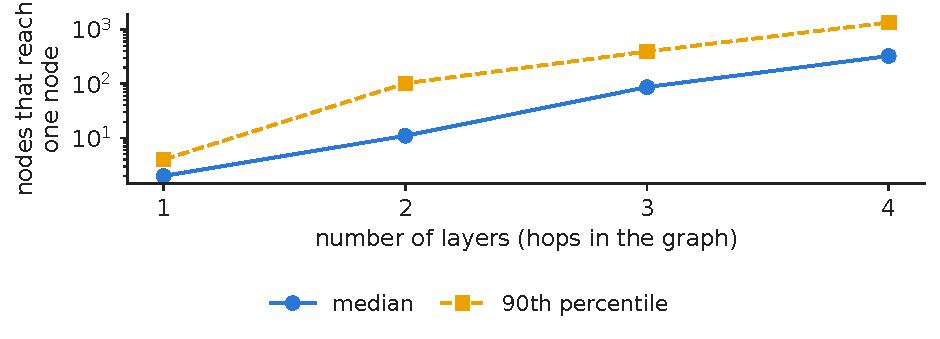
\includegraphics[width=\textwidth,height=0.413\textheight,keepaspectratio]{charts/en/receptive_field.pdf}\end{center}\vspace{-3mm}
\chartsource{Source: Elliptic Bitcoin transaction graph (Weber et al., 2019). Data: Elliptic Bitcoin transaction graph, 49 time steps (about two weeks each).}
\vspace{0.5mm}
\begin{itemize}\setlength{\itemsep}{0pt}
  \item \textbf{Receptive field} of a test transaction: median 2 nodes after 1 layer, 11 after 2, 325 after 4.
  \item \textbf{Tail}: the 90th percentile reaches 1\,356 nodes after 4 layers
    \begin{itemize}\setlength{\itemsep}{0pt}
      \item Hubs connect distant parts of the graph.
    \end{itemize}
\end{itemize}
\par\vfill\manager{$L$ layers = $L$ hops of money flow
    \begin{itemize}\setlength{\itemsep}{0pt}
      \item Two hops already cover most of what an investigator would check by hand.
    \end{itemize}}\par\vspace{0.5mm}
\par\vfill\noindent{\scriptsize\color{FooterGray}(own computation, 2,000 test nodes)}\hfill\qlink{NN\_L9\_receptive\_field}{Quantlets/L9/NN_L9_receptive_field}\par\vspace{0.5mm}
\end{frame}

\begin{frame}{Too many layers make all nodes look alike: over-smoothing}
\small
\begin{center}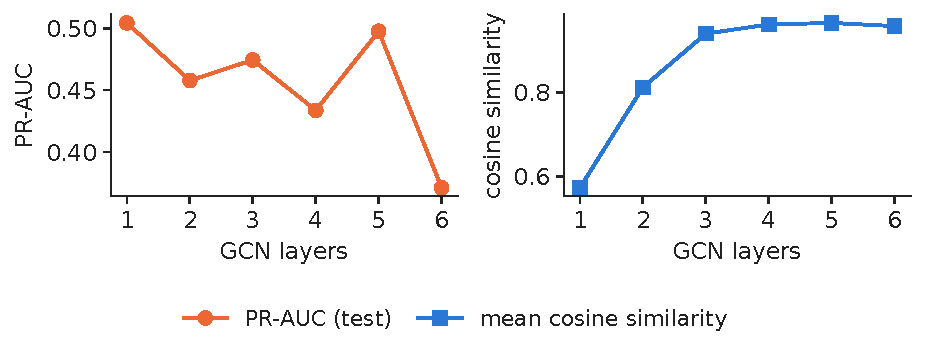
\includegraphics[width=\textwidth,height=0.437\textheight,keepaspectratio]{charts/en/oversmoothing.pdf}\end{center}\vspace{-3mm}
\chartsource{Source: Elliptic Bitcoin transaction graph (Weber et al., 2019). Data: own estimates; training steps 1-34, test time steps 35-49.}
\vspace{0.5mm}
\begin{itemize}\setlength{\itemsep}{0pt}
  \item \textbf{Accuracy}: PR-AUC 0.504 with 1 GCN layer, 0.458 with 2, 0.371 with 6
    \begin{itemize}\setlength{\itemsep}{0pt}
      \item Best depth 1.
    \end{itemize}
  \item \textbf{Similarity}: mean cosine similarity of node representations rises from 0.57 (1 layer) to 0.96 (6 layers)
    \begin{itemize}\setlength{\itemsep}{0pt}
      \item Repeated averaging drives them to a common vector.
    \end{itemize}
\end{itemize}
\par\vfill\manager{GNNs are shallow by design: two or three layers, then residual links or jumping knowledge if more is needed.}\par\vspace{0.5mm}
\par\vfill\noindent{\scriptsize\color{FooterGray}(own computation, 2 seeds; Li, Han \& Wu, 2018)}\hfill\qlink{NN\_L9\_oversmoothing}{Quantlets/L9/NN_L9_oversmoothing}\par\vspace{0.5mm}
\end{frame}


\section{GCN, GraphSAGE and GAT}

\begin{frame}{GCN: average the neighbours with degree weights, then regress}
\footnotesize
\intuition{A GCN layer is a linear regression on the normalised average of a node and its neighbours, followed by a rectified linear unit (ReLU).}
\begin{columns}[T,onlytextwidth]
\begin{column}{0.53\textwidth}
\[ H^{(l+1)}=\ReLU\big(\hat A\,H^{(l)}W^{(l)}\big) \]\[ \mathbf h_v^{(l+1)}=\ReLU\Big(\sum_{u\in\mathcal N(v)\cup\{v\}}\frac{W^{(l)\top}\mathbf h_u^{(l)}}{\sqrt{\tilde d_u\tilde d_v}}\Big) \]{\footnotesize\begin{itemize}\setlength{\itemsep}{0pt}
  \item \textbf{\txtwhere}
    \begin{itemize}\setlength{\itemsep}{0pt}
      \item $H^{(l)}\in\R^{n\times d_l}$ = node representations, $H^{(0)}=\mathbf X$
      \item $W^{(l)}$ = weights shared by all nodes
      \item $\ReLU(x)=\max(0,x)$
      \item Output: $\softmax(\hat A H^{(1)}W^{(2)})$.
    \end{itemize}
\end{itemize}\par}
\end{column}
\begin{column}{0.44\textwidth}
\begin{itemize}\setlength{\itemsep}{3pt}
  \item \textbf{Our GCN}
    \begin{itemize}\setlength{\itemsep}{0pt}
      \item 2 layers, 100 hidden units, dropout 0.2: 26\,902 parameters
      \item Full-batch training on the whole graph, 66 s per seed on the processor (CPU)
    \end{itemize}
  \item \textbf{Cost}
    \begin{itemize}\setlength{\itemsep}{0pt}
      \item $O(|\mathcal E|\,d_l+n\,d_l d_{l+1})$ per layer: linear in the edges
    \end{itemize}
\end{itemize}
\end{column}
\end{columns}
\par\vfill\manager{a GCN is the graph analogue of a moving average: robust, cheap, and blind to which neighbour matters most.}\par\vspace{0.5mm}
\par\vfill\noindent{\scriptsize\color{FooterGray}(Kipf \& Welling, 2017)}\hfill\tryit{notebook \S3}\par\vspace{0.5mm}
\end{frame}

\begin{frame}{GraphSAGE: keep yourself apart from your neighbours, and sample them}
\footnotesize
\intuition{GraphSAGE concatenates a node's own state with the mean of a sample of its neighbours, so it also works on nodes never seen in training.}
\begin{columns}[T,onlytextwidth]
\begin{column}{0.53\textwidth}
\[ \mathbf h_v^{(l+1)}=\ReLU\Big(W_1^{(l)}\mathbf h_v^{(l)}+W_2^{(l)}\frac{1}{|\mathcal S(v)|}\sum_{u\in\mathcal S(v)}\mathbf h_u^{(l)}\Big) \]{\footnotesize\begin{itemize}\setlength{\itemsep}{0pt}
  \item \textbf{\txtwhere}
    \begin{itemize}\setlength{\itemsep}{0pt}
      \item $\mathcal S(v)\subseteq\mathcal N(v)$ = a random sample of at most $k$ neighbours (all of them in our full-batch run)
      \item $W_1$, $W_2$ = separate weights for the node and for its neighbourhood.
    \end{itemize}
\end{itemize}\par}
\end{column}
\begin{column}{0.44\textwidth}
\begin{itemize}\setlength{\itemsep}{3pt}
  \item \textbf{Inductive}
    \begin{itemize}\setlength{\itemsep}{0pt}
      \item The weights do not depend on the graph: tomorrow's transactions get a score without retraining
    \end{itemize}
  \item \textbf{Scalable}
    \begin{itemize}\setlength{\itemsep}{0pt}
      \item Mini-batches of $k$-hop samples: cost bounded by $k^L$ per node, not by the hub degree
    \end{itemize}
  \item \textbf{On Elliptic}
    \begin{itemize}\setlength{\itemsep}{0pt}
      \item Illicit F1 0.564 (sd 0.022), PR-AUC 0.582
    \end{itemize}
\end{itemize}
\end{column}
\end{columns}
\par\vfill\manager{payment systems that score transactions in real time need inductive layers such as GraphSAGE.}\par\vspace{0.5mm}
\par\vfill\noindent{\scriptsize\color{FooterGray}(Hamilton, Ying \& Leskovec, 2017)}\hfill\tryit{notebook \S4}\par\vspace{0.5mm}
\end{frame}

\begin{frame}{GAT: let the network decide which neighbour matters}
\footnotesize
\intuition{A graph attention layer weights each neighbour by a learned score: the attention of Lecture 7, restricted to the edges of the graph.}
\begin{columns}[T,onlytextwidth]
\begin{column}{0.56\textwidth}
\[ \alpha_{vu}=\frac{\exp\big(\mathrm{LeakyReLU}(\mathbf a^{\top}[W\mathbf h_v\,\|\,W\mathbf h_u])\big)}{\sum_{k\in\mathcal N(v)\cup\{v\}}\exp\big(\mathrm{LeakyReLU}(\mathbf a^{\top}[W\mathbf h_v\,\|\,W\mathbf h_k])\big)} \]\[ \mathbf h_v^{(l+1)}=\big\|_{k=1}^{K}\ \ReLU\Big(\sum_{u}\alpha_{vu}^{k}W^{k}\mathbf h_u\Big) \]{\footnotesize\begin{itemize}\setlength{\itemsep}{0pt}
  \item \textbf{\txtwhere}
    \begin{itemize}\setlength{\itemsep}{0pt}
      \item $\mathbf a$ = attention vector
      \item $\|$ = concatenation
      \item $K$ = number of heads (4 here)
      \item Weights $\alpha_{vu}$ sum to one over the neighbours of $v$.
    \end{itemize}
\end{itemize}\par}
\end{column}
\begin{column}{0.41\textwidth}
\begin{itemize}\setlength{\itemsep}{3pt}
  \item \textbf{Link with transformers}
    \begin{itemize}\setlength{\itemsep}{0pt}
      \item A transformer is a GAT on the complete graph of the tokens
    \end{itemize}
  \item \textbf{On Elliptic}
    \begin{itemize}\setlength{\itemsep}{0pt}
      \item 27\,302 parameters; illicit F1 0.489, PR-AUC 0.496
    \end{itemize}
\end{itemize}
\end{column}
\end{columns}
\par\vfill\manager{attention weights are a first, not a final, explanation: they show where the model looked, not why.}\par\vspace{0.5mm}
\par\vfill\noindent{\scriptsize\color{FooterGray}(Veličković et al., 2018)}\hfill\tryit{notebook \S4}\par\vspace{0.5mm}
\end{frame}

\begin{frame}{Training on one big graph: masks, class weights, early stopping}
\footnotesize
\intuition{All nodes pass messages, but only labelled training nodes enter the loss; validation steps decide when to stop.}
\begin{columns}[T,onlytextwidth]
\begin{column}{0.53\textwidth}
\[ \loss(\btheta)=-\frac{1}{|\mathcal V_{tr}|}\sum_{v\in\mathcal V_{tr}}\big[w_1\,y_v\log\hat p_v+w_0(1-y_v)\log(1-\hat p_v)\big] \]{\footnotesize\begin{itemize}\setlength{\itemsep}{0pt}
  \item \textbf{\txtwhere}
    \begin{itemize}\setlength{\itemsep}{0pt}
      \item $\mathcal V_{tr}$ = labelled nodes of steps 1--29
      \item $\hat p_v$ = predicted probability of illicit
      \item $w_1=0.7$, $w_0=0.3$ = class weights of Weber et al.\ (2019)
      \item Adam, learning rate 0.003, weight decay $5\cdot10^{-4}$.
    \end{itemize}
\end{itemize}\par}
\end{column}
\begin{column}{0.44\textwidth}
\begin{itemize}\setlength{\itemsep}{3pt}
  \item \textbf{Validation}
    \begin{itemize}\setlength{\itemsep}{0pt}
      \item Labelled nodes of steps 30--34: best epoch by PR-AUC, patience 40
      \item Median best epoch of the GCN: 47
    \end{itemize}
  \item \textbf{Leakage-free scaling}
    \begin{itemize}\setlength{\itemsep}{0pt}
      \item Feature means and standard deviations from steps 1--34 only
    \end{itemize}
\end{itemize}
\end{column}
\end{columns}
\par\vfill\manager{the unknown nodes are not wasted: they carry messages between labelled ones (semi-supervised learning).}\par\vspace{0.5mm}
\par\vfill\noindent{\scriptsize\color{FooterGray}(Kipf \& Welling, 2017; Weber et al., 2019)}\hfill\tryit{notebook \S3}\par\vspace{0.5mm}
\end{frame}


\section{Case study: illicit Bitcoin transactions}

\begin{frame}{Eight models, one temporal test}
\footnotesize
{\scriptsize\renewcommand{\arraystretch}{1.05}\setlength{\tabcolsep}{4pt}
\begin{tabular}{@{}p{0.27\textwidth}p{0.66\textwidth}@{}}\toprule
Model & What it sees \\ \midrule
Logistic regression & local features only (93), then all 165 \\
Random forest & all features; 100 trees, 50 features per split (Weber et al., 2019) \\
MLP (no graph) & all features, same layers as the GCN but no messages: isolates the value of the edges \\
GCN, GraphSAGE, GAT & all features + the graph; 2 layers, 100 units \\
Random forest + GCN & all features + the 100 hidden GCN outputs of each node \\
\bottomrule\end{tabular}}
\vspace{1mm}
\begin{itemize}\setlength{\itemsep}{2pt}
  \item \textbf{Metrics on steps 35--49}: illicit-class precision, recall and F1 at threshold 0.5
    \begin{itemize}\setlength{\itemsep}{0pt}
      \item PR-AUC (threshold-free).
    \end{itemize}
  \item \textbf{Uncertainty}: 3 seeds per network and per forest
    \begin{itemize}\setlength{\itemsep}{0pt}
      \item Bootstrap of the test nodes for the differences.
    \end{itemize}
\end{itemize}
\par\vfill\noindent{\scriptsize\color{FooterGray}(Weber et al., 2019)}\hfill\tryit{notebook \S2}\par\vspace{0.5mm}
\end{frame}

\begin{frame}{On Elliptic the forest leads; graph layers mainly add ranking power to a network}
\small
\begin{center}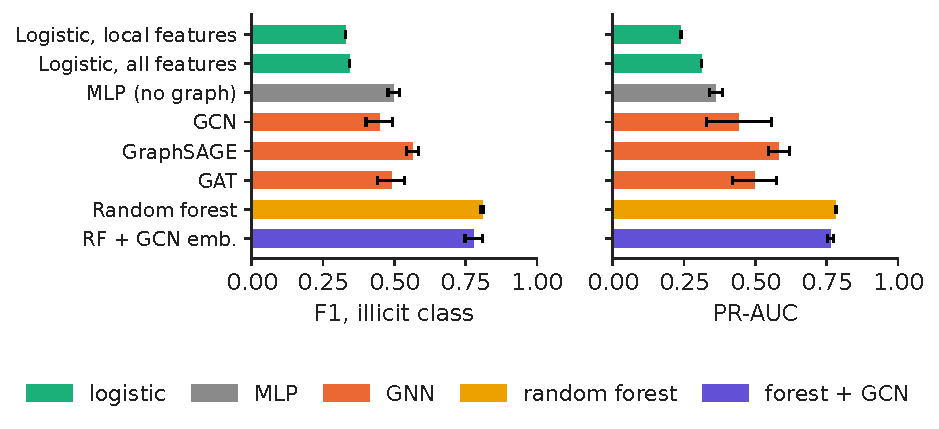
\includegraphics[width=\textwidth,height=0.560\textheight,keepaspectratio]{charts/en/model_comparison.pdf}\end{center}\vspace{-3mm}
\chartsource{Source: Elliptic Bitcoin transaction graph (Weber et al., 2019). Data: own estimates; training steps 1-34, test time steps 35-49.}
\vspace{0.5mm}
\begin{itemize}\setlength{\itemsep}{0pt}
  \item \textbf{Illicit F1}: random forest 0.808, forest + GCN 0.778, GCN 0.447, MLP 0.498, logistic 0.343.
  \item \textbf{Value of the edges}: PR-AUC of the GCN minus the MLP, same layers: \ensuremath{+}8.1 points.
\end{itemize}
\par\vfill\noindent{\scriptsize\color{FooterGray}(own computation; mean $\pm$ sd over 3 seeds)}\hfill\qlink{NN\_L9\_model\_comparison}{Quantlets/L9/NN_L9_model_comparison}\par\vspace{0.5mm}
\end{frame}

\begin{frame}{Precision, recall and the cost of training}
\footnotesize
\begin{columns}[T,onlytextwidth]
\begin{column}{0.56\textwidth}
{\scriptsize\renewcommand{\arraystretch}{1.05}\setlength{\tabcolsep}{4pt}
\begin{tabular}{@{}lrrrrr@{}}\toprule
Model & Prec. & Recall & F1 & PR-AUC & Sec. \\ \midrule
Logistic, local & 0.208 & 0.789 & \cellcolor{Crimson!55}0.329 & \cellcolor{Crimson!55}0.239 & 0.8 \\
Logistic, all & 0.220 & 0.771 & \cellcolor{Crimson!52}0.343 & \cellcolor{Crimson!40}0.311 & 1.8 \\
MLP & 0.517 & 0.483 & \cellcolor{Crimson!16}0.498 & \cellcolor{Crimson!30}0.361 & 59.2 \\
GCN & 0.484 & 0.494 & \cellcolor{Crimson!28}0.447 & \cellcolor{Crimson!14}0.442 & 65.5 \\
GraphSAGE & 0.569 & 0.561 & \cellcolor{Crimson!1}0.564 & \cellcolor{Forest!14}0.582 & 143.2 \\
GAT & 0.488 & 0.500 & \cellcolor{Crimson!18}0.489 & \cellcolor{Crimson!3}0.496 & 231.2 \\
Random forest & 0.914 & 0.725 & \cellcolor{Forest!55}0.808 & \cellcolor{Forest!55}0.782 & 4.9 \\
Forest + GCN & 0.933 & 0.668 & \cellcolor{Forest!48}0.778 & \cellcolor{Forest!51}0.763 & 186.0 \\
\bottomrule\end{tabular}}
\end{column}
\begin{column}{0.41\textwidth}
\begin{itemize}\setlength{\itemsep}{3pt}
  \item \textbf{Reading the table}
    \begin{itemize}\setlength{\itemsep}{0pt}
      \item Precision = share of alerts that are illicit; recall = share of illicit found
      \item Green = best, red = worst in the column
    \end{itemize}
  \item \textbf{Forest}
    \begin{itemize}\setlength{\itemsep}{0pt}
      \item Precision 0.914, recall 0.725
    \end{itemize}
  \item \textbf{Logistic, class weights 0.3/0.7}
    \begin{itemize}\setlength{\itemsep}{0pt}
      \item Precision 0.220, recall 0.771: the weights buy recall with false alarms
    \end{itemize}
\end{itemize}
\end{column}
\end{columns}
\par\vfill\manager{the right model depends on what an error costs: a missed laundering case or an analyst's wasted hour.}\par\vspace{0.5mm}
\par\vfill\noindent{\scriptsize\color{FooterGray}(own computation; sec.\ = training time per seed, CPU)}\hfill\tryit{notebook \S2}\par\vspace{0.5mm}
\end{frame}

\begin{frame}{Precision-recall curves: the ranking behind the F1}
\small
\begin{center}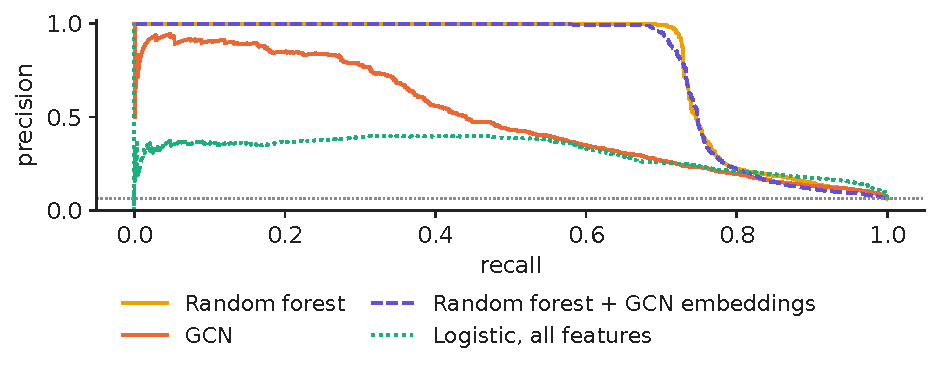
\includegraphics[width=\textwidth,height=0.580\textheight,keepaspectratio]{charts/en/pr_curves.pdf}\end{center}\vspace{-3mm}
\chartsource{Source: Elliptic Bitcoin transaction graph (Weber et al., 2019). Data: own estimates; training steps 1-34, test time steps 35-49.}
\vspace{0.5mm}
\begin{itemize}\setlength{\itemsep}{0pt}
  \item \textbf{PR-AUC}: random forest 0.782, forest + GCN 0.763, GCN 0.442, logistic 0.311
    \begin{itemize}\setlength{\itemsep}{0pt}
      \item A random score would give 6.50\,\% (dotted line).
    \end{itemize}
\end{itemize}
\par\vfill\noindent{\scriptsize\color{FooterGray}$\text{PR-AUC}=\sum_k (R_k-R_{k-1})P_k$}\hfill\qlink{NN\_L9\_pr\_curves}{Quantlets/L9/NN_L9_pr_curves}\par\vspace{0.5mm}
\end{frame}

\begin{frame}{Is the gap real? A bootstrap of the test transactions}
\footnotesize
\intuition{One test set gives one number; resampling the test nodes shows how much that number could move.}
\begin{columns}[T,onlytextwidth]
\begin{column}{0.53\textwidth}
\[ \Delta^{*b}=\text{PR-AUC}_A\big(\mathcal T^{*b}\big)-\text{PR-AUC}_B\big(\mathcal T^{*b}\big),\quad b=1,\dots,B \]\[ \text{CI}_{95\%}=\big[q_{0.025}(\Delta^{*}),\ q_{0.975}(\Delta^{*})\big] \]{\footnotesize\begin{itemize}\setlength{\itemsep}{0pt}
  \item \textbf{\txtwhere}
    \begin{itemize}\setlength{\itemsep}{0pt}
      \item $\mathcal T^{*b}$ = test nodes drawn with replacement
      \item $B=1{,}000$
      \item Scores = mean over 3 seeds
      \item The same draw is used for both models (paired).
    \end{itemize}
\end{itemize}\par}
\end{column}
\begin{column}{0.44\textwidth}
\begin{itemize}\setlength{\itemsep}{3pt}
  \item \textbf{Forest minus GCN}
    \begin{itemize}\setlength{\itemsep}{0pt}
      \item $\Delta$ = 0.285, 95\,\% interval [0.259; 0.313]
    \end{itemize}
  \item \textbf{Forest + GCN minus forest}
    \begin{itemize}\setlength{\itemsep}{0pt}
      \item $\Delta$ = \ensuremath{-}0.008, 95\,\% interval [\ensuremath{-}0.015; \ensuremath{-}0.002]
    \end{itemize}
  \item an interval that excludes 0 supports a real difference on this test period
\end{itemize}
\end{column}
\end{columns}
\par\vfill\manager{report the interval, not only the winner: a fraud committee decides on ranges, not on the third decimal.}\par\vspace{0.5mm}
\par\vfill\noindent{\scriptsize\color{FooterGray}(Efron \& Tibshirani, 1993)}\hfill\tryit{notebook \S2}\par\vspace{0.5mm}
\end{frame}

\begin{frame}{Why the forest is hard to beat here: its features already pass messages}
\footnotesize
\begin{columns}[T,onlytextwidth]
\begin{column}{0.49\textwidth}
\begin{itemize}\setlength{\itemsep}{4pt}
  \item \textbf{Hand-made message passing}
    \begin{itemize}\setlength{\itemsep}{0pt}
      \item 72 of the 165 features are aggregates over the one-hop neighbours (max, min, sd, correlation)
      \item This is one fixed GNN layer, computed by Elliptic before release
    \end{itemize}
  \item \textbf{Local features only}
    \begin{itemize}\setlength{\itemsep}{0pt}
      \item Logistic regression F1 0.329 vs 0.343 with the aggregates
    \end{itemize}
  \item \textbf{Trees}
    \begin{itemize}\setlength{\itemsep}{0pt}
      \item Thresholds on amounts and counts fit fraud patterns that are rules (``more than $k$ inputs'')
    \end{itemize}
\end{itemize}
\end{column}
\begin{column}{0.48\textwidth}
\begin{itemize}\setlength{\itemsep}{4pt}
  \item \textbf{Where GNNs earn their keep}
    \begin{itemize}\setlength{\itemsep}{0pt}
      \item Raw graphs without engineered aggregates
      \item Multi-hop patterns (layering through many accounts)
      \item Inductive scoring of new nodes, and embeddings for other models
    \end{itemize}
  \item \textbf{Combine}
    \begin{itemize}\setlength{\itemsep}{0pt}
      \item Forest + GCN representations: F1 change \ensuremath{-}3.0 points
    \end{itemize}
\end{itemize}
\end{column}
\end{columns}
\par\vfill\manager{before training a GNN, check whether the data provider has already aggregated the neighbourhood for you.}\par\vspace{0.5mm}
\par\vfill\noindent{\scriptsize\color{FooterGray}(Weber et al., 2019)}\hfill\tryit{notebook \S2}\par\vspace{0.5mm}
\end{frame}

\begin{frame}{A dark-market shutdown breaks every model: concept drift}
\small
\begin{center}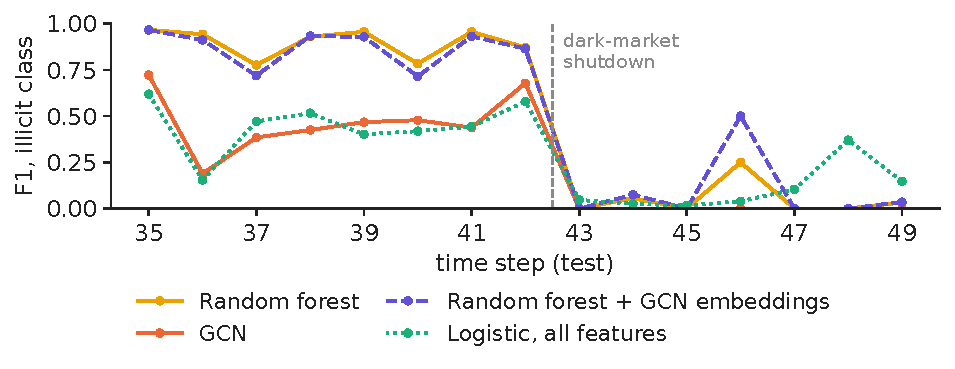
\includegraphics[width=\textwidth,height=0.415\textheight,keepaspectratio]{charts/en/f1_by_timestep.pdf}\end{center}\vspace{-3mm}
\chartsource{Source: Elliptic Bitcoin transaction graph (Weber et al., 2019). Data: own estimates; training steps 1-34, test time steps 35-49.}
\vspace{0.5mm}
\begin{itemize}\setlength{\itemsep}{0pt}
  \item \textbf{Before step 43}: mean F1 random forest 0.898, GCN 0.473
    \begin{itemize}\setlength{\itemsep}{0pt}
      \item \textbf{from step 43}: 0.048 and 0.000.
    \end{itemize}
  \item \textbf{New behaviour}: after a major dark market closed, illicit flows changed form
    \begin{itemize}\setlength{\itemsep}{0pt}
      \item No model trained on steps 1--34 had seen it (Weber et al., 2019).
    \end{itemize}
\end{itemize}
\par\vfill\manager{monitor F1 per period and retrain on recent labels
    \begin{itemize}\setlength{\itemsep}{0pt}
      \item A static AML model ages within weeks.
    \end{itemize}}\par\vspace{0.5mm}
\par\vfill\noindent{\scriptsize\color{FooterGray}}\hfill\qlink{NN\_L9\_f1\_by\_timestep}{Quantlets/L9/NN_L9_f1_by_timestep}\par\vspace{0.5mm}
\end{frame}

\begin{frame}{What an investigation team gets from 1,000 alerts}
\small
\begin{center}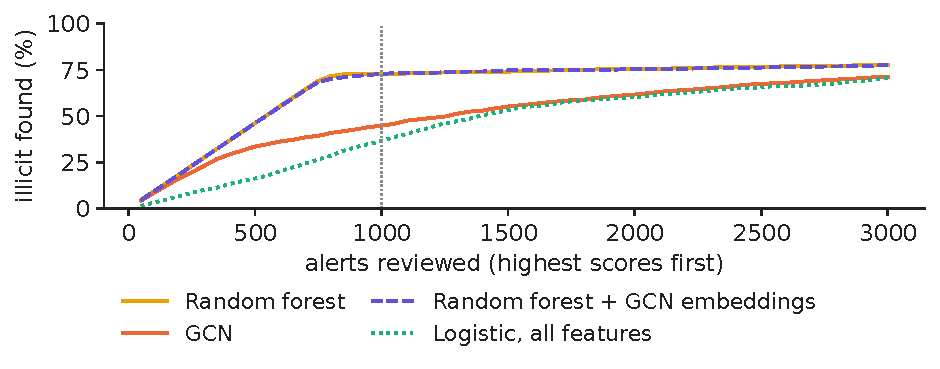
\includegraphics[width=\textwidth,height=0.443\textheight,keepaspectratio]{charts/en/alert_budget.pdf}\end{center}\vspace{-3mm}
\chartsource{Source: Elliptic Bitcoin transaction graph (Weber et al., 2019). Data: own estimates; training steps 1-34, test time steps 35-49.}
\vspace{0.5mm}
\begin{itemize}\setlength{\itemsep}{0pt}
  \item \textbf{Top 1\,000 scores} of the test period contain 72.9\,\% of all illicit transactions for the random forest, 44.8\,\% for the GCN, 72.9\,\% for forest + GCN.
  \item \textbf{Hit rate} of those alerts: 78.9\,\% (forest), 48.5\,\% (GCN), out of 1\,083 illicit test transactions.
\end{itemize}
\par\vfill\manager{size the team from this curve: the alert budget, not the F1, is the constraint in a compliance department.}\par\vspace{0.5mm}
\par\vfill\noindent{\scriptsize\color{FooterGray}}\hfill\qlink{NN\_L9\_alert\_budget}{Quantlets/L9/NN_L9_alert_budget}\par\vspace{0.5mm}
\end{frame}

\begin{frame}{The GCN learns a space where illicit transactions gather}
\small
\begin{center}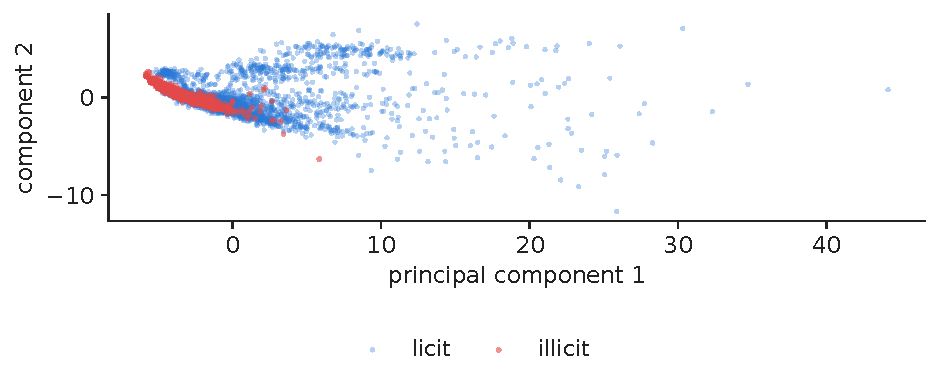
\includegraphics[width=\textwidth,height=0.550\textheight,keepaspectratio]{charts/en/gcn_embeddings.pdf}\end{center}\vspace{-3mm}
\chartsource{Source: Elliptic Bitcoin transaction graph (Weber et al., 2019). Data: own estimates; training steps 1-34, test time steps 35-49.}
\vspace{0.5mm}
\begin{itemize}\setlength{\itemsep}{0pt}
  \item \textbf{Hidden layer} of the GCN (100 dimensions) projected by principal component analysis (PCA) on its first two components: 79.2\,\% of the variance.
  \item \textbf{Reuse}: these vectors are the inputs of the forest + GCN model and can feed any other risk model.
\end{itemize}
\par\vfill\noindent{\scriptsize\color{FooterGray}(own computation; 1\,083 illicit and 3,000 licit test nodes)}\hfill\qlink{NN\_L9\_gcn\_embeddings}{Quantlets/L9/NN_L9_gcn_embeddings}\par\vspace{0.5mm}
\end{frame}

\begin{frame}{Adding graph features reshuffles the explanations}
\small
\begin{center}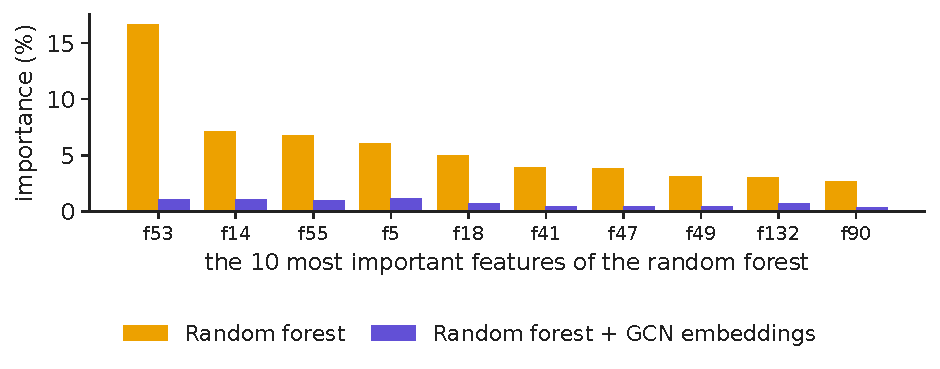
\includegraphics[width=\textwidth,height=0.407\textheight,keepaspectratio]{charts/en/importance_shift.pdf}\end{center}\vspace{-3mm}
\chartsource{Source: Elliptic Bitcoin transaction graph (Weber et al., 2019). Data: own estimates; training steps 1-34, test time steps 35-49.}
\vspace{0.5mm}
\begin{itemize}\setlength{\itemsep}{0pt}
  \item \textbf{Importance mass}: the 10 top features of the forest carry 58.2\,\% of the importance
    \begin{itemize}\setlength{\itemsep}{0pt}
      \item With GCN embeddings they keep 7.4\,\%, the embeddings take 73.9\,\%.
    \end{itemize}
  \item \textbf{Stability across 3 refits}: mean Spearman correlation of the importances 0.973 (forest) and 0.896 (forest + GCN).
\end{itemize}
\par\vfill\manager{compare explanations across refits before reading a change of model as a change of explanation (next: research from our group).}\par\vspace{0.5mm}
\par\vfill\noindent{\scriptsize\color{FooterGray}}\hfill\qlink{NN\_L9\_importance\_shift}{Quantlets/L9/NN_L9_importance_shift}\par\vspace{0.5mm}
\end{frame}


\section{GNNs in production}

\begin{frame}{Four pitfalls of graph models in finance}
\footnotesize
\begin{columns}[T,onlytextwidth]
\begin{column}{0.49\textwidth}
\begin{itemize}\setlength{\itemsep}{5pt}
  \item \textbf{Leakage through edges}
    \begin{itemize}\setlength{\itemsep}{0pt}
      \item A test node must not receive messages from the future
      \item In Elliptic 100.0\,\% of the edges stay inside one time step, so the temporal split is clean
    \end{itemize}
  \item \textbf{Few labels}
    \begin{itemize}\setlength{\itemsep}{0pt}
      \item Only 22.9\,\% of the nodes are labelled; labels come from past investigations and are biased towards cases already found
    \end{itemize}
\end{itemize}
\end{column}
\begin{column}{0.48\textwidth}
\begin{itemize}\setlength{\itemsep}{5pt}
  \item \textbf{Drift}
    \begin{itemize}\setlength{\itemsep}{0pt}
      \item Criminals adapt: the shutdown at step 43 changed the patterns
      \item Temporal GNNs (EvolveGCN) let the weights evolve with time
    \end{itemize}
  \item \textbf{Explainability}
    \begin{itemize}\setlength{\itemsep}{0pt}
      \item A suspicious-activity report needs a reason a regulator can read
      \item GNNExplainer finds the subgraph and features behind one prediction
    \end{itemize}
\end{itemize}
\end{column}
\end{columns}
\par\vfill\manager{test a graph model the way it will run: on later periods, with the labels available at that time.}\par\vspace{0.5mm}
\par\vfill\noindent{\scriptsize\color{FooterGray}(Pareja et al., 2020; Ying et al., 2019)}\par\vspace{0.5mm}
\end{frame}

\begin{frame}{Graphs everywhere in finance}
\footnotesize
\begin{columns}[T,onlytextwidth]
\begin{column}{0.49\textwidth}
\begin{itemize}\setlength{\itemsep}{5pt}
  \item \textbf{Payments and cards}
    \begin{itemize}\setlength{\itemsep}{0pt}
      \item Cardholder--merchant graphs: a compromised terminal links many fraud victims
    \end{itemize}
  \item \textbf{Credit}
    \begin{itemize}\setlength{\itemsep}{0pt}
      \item Guarantor and supplier networks: default spreads along trade credit
    \end{itemize}
  \item \textbf{Crypto}
    \begin{itemize}\setlength{\itemsep}{0pt}
      \item Address and transaction graphs (this lecture), mixer detection, wallet clustering
    \end{itemize}
\end{itemize}
\end{column}
\begin{column}{0.48\textwidth}
\begin{itemize}\setlength{\itemsep}{5pt}
  \item \textbf{Systemic risk}
    \begin{itemize}\setlength{\itemsep}{0pt}
      \item Interbank exposures and tail-dependence networks: who falls if one bank fails
    \end{itemize}
  \item \textbf{Markets}
    \begin{itemize}\setlength{\itemsep}{0pt}
      \item Graphs of stocks linked by correlation, supply chain or ownership, for return forecasts
    \end{itemize}
  \item \textbf{Energy}
    \begin{itemize}\setlength{\itemsep}{0pt}
      \item Power grids and interconnected price zones are graphs by construction
    \end{itemize}
\end{itemize}
\end{column}
\end{columns}
\par\vfill\manager{whenever the risk of one unit depends on its counterparties, a graph model is worth a try.}\par\vspace{0.5mm}
\par\vfill\noindent{\scriptsize\color{FooterGray}(Hamilton, 2020; Bishop \& Bishop, 2024, ch.\ 13)}\par\vspace{0.5mm}
\end{frame}


\section{Wrap-up}

\begin{frame}{What to remember}
\small
\begin{itemize}\setlength{\itemsep}{6pt}
  \item \textbf{A GNN layer} = message, permutation-invariant aggregation, update
    \begin{itemize}\setlength{\itemsep}{0pt}
      \item GCN averages with degree weights, GraphSAGE separates self and neighbours, GAT learns the weights.
    \end{itemize}
  \item \textbf{Depth} = hops: two layers reach a median of 11 transactions
    \begin{itemize}\setlength{\itemsep}{0pt}
      \item More layers over-smooth (PR-AUC 0.371 with 6 layers).
    \end{itemize}
  \item \textbf{On Elliptic} the edges help a network (GCN vs MLP: \ensuremath{+}8.1 PR-AUC points), but a random forest on pre-aggregated features leads (F1 0.808).
  \item \textbf{Judge AML models} on later periods, with PR-AUC, alert budgets and bootstrap intervals
    \begin{itemize}\setlength{\itemsep}{0pt}
      \item Watch drift and the stability of explanations.
    \end{itemize}
\end{itemize}
\end{frame}

\begin{frame}{Research from our group: graphs, fraud and explanations}
\footnotesize
\begin{itemize}\setlength{\itemsep}{5pt}
  \item \textbf{Explanation stability in graph-augmented fraud detection} (Diaconu \& Pele, 2026): treats the complete model refit as the unit of inference and compares SHapley Additive exPlanations (SHAP) of fraud models with and without graph embeddings against graph-free controls matched in dimension and covariance.
  \item \textbf{Key results}: augmentation can shrink the attributions of the original features mechanically
    \begin{itemize}\setlength{\itemsep}{0pt}
      \item After accounting for retraining variability, graph-free controls reproduce most of the movement in marginal SHAP stability, while local, row-level rankings change.
    \end{itemize}
  \item \textbf{Energy Financial Risk Meter} (Toma, Dima, Grecu, Pele \& Lessmann, 2026): measures systemic risk in the European Union energy sector from the network of tail dependencies between firms.
\end{itemize}
\vspace{1mm}{\scriptsize Findings as stated in the papers; the numbers on the other slides come from our own computations.}
\par\vfill\noindent{\scriptsize\color{FooterGray}(Bucharest University of Economic Studies; Romanian Academy, Institute for Economic Forecasting)}\par\vspace{0.5mm}
\end{frame}

\begin{frame}{Want to learn more?}
\small
\begin{columns}[T,onlytextwidth]
\begin{column}{0.52\textwidth}
\begin{itemize}\setlength{\itemsep}{4pt}
  \item \textbf{Bishop \& Bishop (2024)}, chapter 13: graph neural networks, from message passing to graph attention.
  \item \textbf{Hamilton (2020)}, \textit{Graph Representation Learning}, free draft: \href{https://www.cs.mcgill.ca/~wlh/grl_book/}{cs.mcgill.ca/\textasciitilde wlh/grl\_book}.
  \item \textbf{PyTorch Geometric} tutorials: \href{https://pytorch-geometric.readthedocs.io}{pytorch-geometric.readthedocs.io}.
\end{itemize}
\end{column}
\begin{column}{0.45\textwidth}
\begin{itemize}\setlength{\itemsep}{4pt}
  \item \textbf{Elliptic data set} and the original paper: \href{https://arxiv.org/abs/1908.02591}{arXiv:1908.02591}.
  \item \textbf{This course}: code, data, notebooks --- \href{https://github.com/danpele/NEURAL_BIZ}{github.com/danpele/NEURAL\_BIZ}.
  \item \textbf{Experiment yourself}: the notebook reproduces every chart and number of this lecture.
\end{itemize}
\end{column}
\end{columns}
\end{frame}

\begin{frame}{Quiz 1: permutations}
\small
\begin{itemize}
  \item We renumber the transactions of the graph.
    \begin{itemize}\setlength{\itemsep}{0pt}
      \item What must happen to the GCN scores?
    \end{itemize}
\end{itemize}
\vspace{2mm}
\begin{exampleblock}{Answer}
\begin{itemize}
  \item They are permuted in the same way and are otherwise unchanged: a GNN layer is permutation-equivariant, because the aggregation over neighbours does not depend on order.
\end{itemize}
\end{exampleblock}
\end{frame}

\begin{frame}{Quiz 2: depth}
\small
\begin{itemize}
  \item Why not stack ten GCN layers to see ten hops of money flow?
\end{itemize}
\vspace{2mm}
\begin{exampleblock}{Answer}
\begin{itemize}
  \item Repeated degree-weighted averaging makes all representations similar (over-smoothing): on Elliptic PR-AUC falls from 0.458 (2 layers) to 0.371 (6 layers).
\end{itemize}
\end{exampleblock}
\end{frame}

\begin{frame}{Quiz 3: the strong benchmark}
\small
\begin{itemize}
  \item Why does a random forest without the graph beat the GCN on Elliptic?
\end{itemize}
\vspace{2mm}
\begin{exampleblock}{Answer}
\begin{itemize}
  \item 72 of its features are already aggregates over the neighbours, a hand-made message-passing layer
    \begin{itemize}\setlength{\itemsep}{0pt}
      \item Trees also fit rule-like fraud thresholds well.
    \end{itemize}
\end{itemize}
\end{exampleblock}
\end{frame}

\begin{frame}{Quiz 4: evaluation}
\small
\begin{itemize}
  \item Only 6.50\,\% of the test transactions are illicit.
    \begin{itemize}\setlength{\itemsep}{0pt}
      \item Which metric would mislead a compliance officer?
    \end{itemize}
\end{itemize}
\vspace{2mm}
\begin{exampleblock}{Answer}
\begin{itemize}
  \item Accuracy: labelling everything licit is right most of the time and finds no criminal
    \begin{itemize}\setlength{\itemsep}{0pt}
      \item Use precision, recall, PR-AUC and the alert budget.
    \end{itemize}
\end{itemize}
\end{exampleblock}
\end{frame}

\begin{frame}{Quiz 5: attention on graphs}
\small
\begin{itemize}
  \item What is the link between a GAT layer and the transformer of Lecture 7?
\end{itemize}
\vspace{2mm}
\begin{exampleblock}{Answer}
\begin{itemize}
  \item Both weight neighbours by a softmax of learned scores
    \begin{itemize}\setlength{\itemsep}{0pt}
      \item A transformer is attention on the complete graph of the tokens, a GAT restricts it to the edges of the graph.
    \end{itemize}
\end{itemize}
\end{exampleblock}
\end{frame}

\begin{frame}{References (1/2)}
\scriptsize
\begin{itemize}\setlength{\itemsep}{0pt}\scriptsize
\item Bishop, C.\,M.\ \& Bishop, H.\ (2024). \textit{Deep Learning: Foundations and Concepts}, ch.\ 13. Springer. \href{https://doi.org/10.1007/978-3-031-45468-4}{doi:10.1007/978-3-031-45468-4}
\item Breiman, L.\ (2001). Random forests. \textit{Machine Learning}, 45(1), 5--32. \href{https://doi.org/10.1023/A:1010933404324}{doi:10.1023/A:1010933404324}
\item Diaconu, D.\ \& Pele, D.\,T.\ (2026). SHAP stability across random and forward-time validation in graph-augmented fraud detection. Submitted to \textit{Expert Systems with Applications}. Code: \href{https://github.com/QuantLet/GNN_XAI_Stability}{github.com/QuantLet/GNN\_XAI\_Stability}
\item Efron, B.\ \& Tibshirani, R.\,J.\ (1993). \textit{An Introduction to the Bootstrap}. Chapman \& Hall. \href{https://doi.org/10.1201/9780429246593}{doi:10.1201/9780429246593}
\item Fey, M.\ \& Lenssen, J.\,E.\ (2019). Fast graph representation learning with PyTorch Geometric. ICLR Workshop on Representation Learning on Graphs and Manifolds. \href{https://arxiv.org/abs/1903.02428}{arXiv:1903.02428}
\item Gilmer, J., Schoenholz, S.\,S., Riley, P.\,F., Vinyals, O.\ \& Dahl, G.\,E.\ (2017). Neural message passing for quantum chemistry. \textit{Proceedings of ICML}, PMLR 70, 1263--1272. \href{https://arxiv.org/abs/1704.01212}{arXiv:1704.01212}
\item Hamilton, W.\,L., Ying, R.\ \& Leskovec, J.\ (2017). Inductive representation learning on large graphs. \textit{Advances in Neural Information Processing Systems}, 30. \href{https://arxiv.org/abs/1706.02216}{arXiv:1706.02216}
\item Hamilton, W.\,L.\ (2020). \textit{Graph Representation Learning}. Morgan \& Claypool. \href{https://doi.org/10.2200/S01045ED1V01Y202009AIM046}{doi:10.2200/S01045ED1V01Y202009AIM046}
\item Kipf, T.\,N.\ \& Welling, M.\ (2017). Semi-supervised classification with graph convolutional networks. \textit{International Conference on Learning Representations}. \href{https://arxiv.org/abs/1609.02907}{arXiv:1609.02907}
\end{itemize}
\end{frame}

\begin{frame}{References (2/2)}
\scriptsize
\begin{itemize}\setlength{\itemsep}{0pt}\scriptsize
\item Li, Q., Han, Z.\ \& Wu, X.-M.\ (2018). Deeper insights into graph convolutional networks for semi-supervised learning. \textit{Proceedings of the AAAI Conference on Artificial Intelligence}, 32(1). \href{https://doi.org/10.1609/aaai.v32i1.11604}{doi:10.1609/aaai.v32i1.11604}
\item Lundberg, S.\,M.\ \& Lee, S.-I.\ (2017). A unified approach to interpreting model predictions. \textit{Advances in Neural Information Processing Systems}, 30. \href{https://arxiv.org/abs/1705.07874}{arXiv:1705.07874}
\item Pareja, A., Domeniconi, G., Chen, J.\ et al.\ (2020). EvolveGCN: Evolving graph convolutional networks for dynamic graphs. \textit{Proceedings of the AAAI Conference on Artificial Intelligence}, 34(4), 5363--5370. \href{https://doi.org/10.1609/aaai.v34i04.5984}{doi:10.1609/aaai.v34i04.5984}
\item Toma, F.-M., Dima, D.-M., Grecu, R., Pele, D.\,T.\ \& Lessmann, S.\ (2026). Energy Financial Risk Meter: Systemic risk in the EU energy sector. SSRN Working Paper 6985301. \href{https://doi.org/10.2139/ssrn.6985301}{doi:10.2139/ssrn.6985301}
\item Veličković, P., Cucurull, G., Casanova, A., Romero, A., Liò, P.\ \& Bengio, Y.\ (2018). Graph attention networks. \textit{International Conference on Learning Representations}. \href{https://arxiv.org/abs/1710.10903}{arXiv:1710.10903}
\item Weber, M., Domeniconi, G., Chen, J., Weidele, D.\,K.\,I., Bellei, C., Robinson, T.\ \& Leiserson, C.\,E.\ (2019). Anti-money laundering in Bitcoin: Experimenting with graph convolutional networks for financial forensics. KDD Workshop on Anomaly Detection in Finance. \href{https://arxiv.org/abs/1908.02591}{arXiv:1908.02591}
\item Xu, K., Hu, W., Leskovec, J.\ \& Jegelka, S.\ (2019). How powerful are graph neural networks? \textit{International Conference on Learning Representations}. \href{https://arxiv.org/abs/1810.00826}{arXiv:1810.00826}
\item Ying, R., Bourgeois, D., You, J., Zitnik, M.\ \& Leskovec, J.\ (2019). GNNExplainer: Generating explanations for graph neural networks. \textit{Advances in Neural Information Processing Systems}, 32. \href{https://arxiv.org/abs/1903.03894}{arXiv:1903.03894}
\end{itemize}
\end{frame}

\appendix

\section*{Appendix}

\begin{frame}{Appendix A: from spectral filters to the GCN layer}
\small
\begin{columns}[T,onlytextwidth]
\begin{column}{0.52\textwidth}
\[ g_\theta\star\mathbf x\approx\sum_{k=0}^{K}\theta_k T_k(\tilde L)\,\mathbf x,\quad \tilde L=\tfrac{2}{\lambda_{\max}}L_{sym}-I \]\[ K=1,\ \lambda_{\max}\approx2:\quad g_\theta\star\mathbf x\approx\theta_0\mathbf x-\theta_1D^{-1/2}AD^{-1/2}\mathbf x \]\[ \theta=\theta_0=-\theta_1:\quad \theta\,(I+D^{-1/2}AD^{-1/2})\,\mathbf x\ \to\ \theta\,\hat A\,\mathbf x \]
\end{column}
\begin{column}{0.45\textwidth}
\begin{itemize}\setlength{\itemsep}{3pt}
  \item $T_k$ = Chebyshev polynomials
    \begin{itemize}\setlength{\itemsep}{0pt}
      \item $L_{sym}=I-D^{-1/2}AD^{-1/2}$
      \item A polynomial of degree $K$ only mixes nodes within $K$ hops.
    \end{itemize}
  \item One shared parameter per feature pair avoids overfitting
    \begin{itemize}\setlength{\itemsep}{0pt}
      \item The renormalisation trick $I+D^{-1/2}AD^{-1/2}\to\tilde D^{-1/2}\tilde A\tilde D^{-1/2}$ keeps eigenvalues in $(-1,1]$.
    \end{itemize}
  \item With $d$ input features and $d'$ outputs, $\theta$ becomes the matrix $W\in\R^{d\times d'}$.
\end{itemize}
\end{column}
\end{columns}
\par\vfill\noindent{\scriptsize\color{FooterGray}(Kipf \& Welling, 2017)}\par\vspace{0.5mm}
\end{frame}

\begin{frame}{Appendix B: the Weisfeiler--Leman test}
\small
\begin{columns}[T,onlytextwidth]
\begin{column}{0.50\textwidth}
\[ c_v^{(l+1)}=\operatorname{hash}\Big(c_v^{(l)},\ \{\!\{c_u^{(l)}:u\in\mathcal N(v)\}\!\}\Big) \]
\end{column}
\begin{column}{0.47\textwidth}
\begin{itemize}\setlength{\itemsep}{3pt}
  \item Start with the same colour for all nodes
    \begin{itemize}\setlength{\itemsep}{0pt}
      \item Refine by hashing each node's colour with the multiset of its neighbours' colours.
    \end{itemize}
  \item Two graphs with different colour histograms are not isomorphic
    \begin{itemize}\setlength{\itemsep}{0pt}
      \item Equal histograms are inconclusive.
    \end{itemize}
  \item A message-passing GNN is at most as discriminative as WL
    \begin{itemize}\setlength{\itemsep}{0pt}
      \item GIN reaches this bound with sum aggregation and an injective update.
    \end{itemize}
\end{itemize}
\end{column}
\end{columns}
\par\vfill\noindent{\scriptsize\color{FooterGray}(Xu et al., 2019)}\par\vspace{0.5mm}
\end{frame}

\begin{frame}{Appendix C: settings of the experiment}
\small
{\scriptsize\renewcommand{\arraystretch}{1.05}\setlength{\tabcolsep}{4pt}
\begin{tabular}{@{}p{0.30\textwidth}p{0.62\textwidth}@{}}\toprule
Setting & Value \\ \midrule
Split & train steps 1--29, validation 30--34, test 35--49 (labelled nodes only in the loss) \\
Networks & 2 layers, 100 units, ReLU, dropout 0.2; GAT: 4 heads of 25; Adam, rate 0.003, decay $5\cdot10^{-4}$; at most 300 epochs, patience 40 \\
Class weights & 0.3 / 0.7 \\
Random forest & 100 trees, 50 features per split, raw features \\
Seeds & 1, 2, 3 \\
Software, hardware & PyTorch, PyTorch Geometric, scikit-learn; laptop CPU, total 0.1 minutes \\
\bottomrule\end{tabular}}
\par\vfill\noindent{\scriptsize\color{FooterGray}(Weber et al., 2019; Fey \& Lenssen, 2019)}\par\vspace{0.5mm}
\end{frame}

\end{document}
